\chapter{Implementación}
\label{cap: capitulo_5}

\begin{quote}
	\small \flushright ''\textit{Hay varias formas de hacer las cosas, y una de ellas es hacerlas bien.}'' \\
	--- Profesora Mª Amparo Vila Miranda (2010).
\end{quote}

\vspace{8em}

A lo largo de este capítulo vamos a explicar cómo hemos llevado a cabo el proceso de implementación del sistema, partiendo del diseño especificado en las páginas anteriores.

Todos los bloques se han implantado con una filosofía similar, teniendo en cuenta que nos dirigimos a un \textbf{sistema empotrado}, de prestaciones limitadas, y donde la \textbf{seguridad} y el \textbf{tiempo de respuesta} son cruciales.

Debemos tener también en cuenta que el servicio podrá ser utilizado por \textbf{varios usuarios} a la vez ---incluso varios componentes--- y el planificador, si bien no requiere características de tiempo-real estricto, es necesario que responda adecuadamente a los tiempos marcados por la partitura.

En el demonio, nuestra máxima prioridad será la \textbf{eficiencia}, mientras que en la interfaz \textit{web} nos centraremos en la \textbf{accesibilidad}.

\newpage

\section{Servicio del reproductor}

Este bloque compone el \textit{back-end} del sistema. Comprende una gran cantidad de elementos técnicos y hace uso de numerosas funciones del sistema operativo. Vamos a escribirlo casi por completo en \textbf{lenguaje C}, por las siguientes razones:

\begin{enumerate}
	\item Alta calidad y \textbf{eficiencia}.
	\item Cercanía al \textbf{\textit{hardware}}.
	\item Capacidad para hacer \textbf{llamadas al sistema} Linux.
	\item Posibilidad de acceder al código ensamblador para hacer \textbf{optimizaciones}.
\end{enumerate}

Aunque todos los ejecutables se van a compilar desde código \textit{C}, haremos uso de \textit{shell-scripts} y un \textit{Makefile} que nos permitirá compilar fácilmente las fuentes e instalar los ejecutables.

En ciertos componentes, necesitaremos hacer \textbf{prototipos} para estudiar su funcionamiento y realizar pruebas de concepto, antes de implantarlos definitivamente. Esto lo haremos en \textbf{Python}, un lenguaje interpretado y de programación más ágil que C.

En resumen, utilizaremos el siguiente procedimiento con los componentes más complejos, que así lo requieran:

\smallskip

\begin{figure}[H]
	\noindent \begin{centering}
		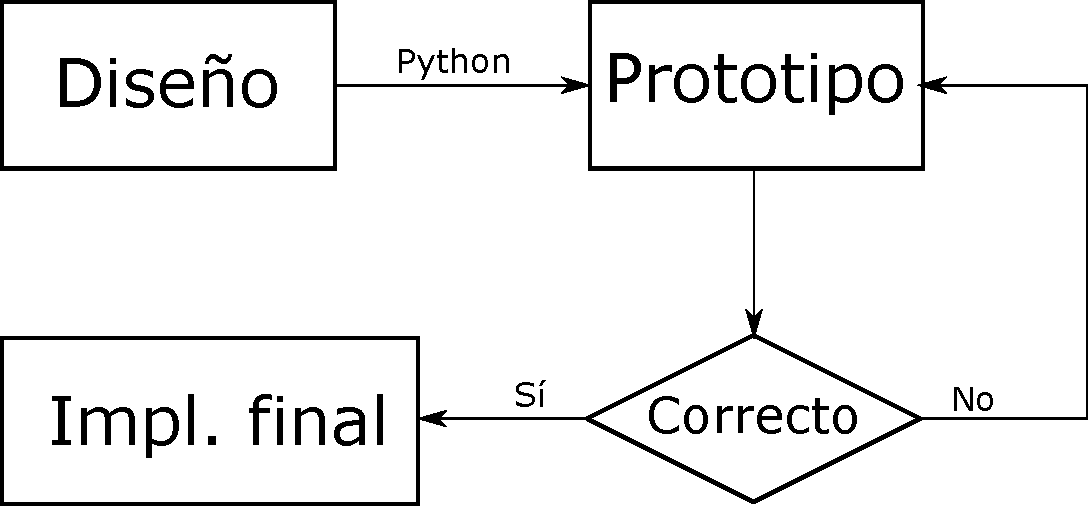
\includegraphics[width=\linewidth/2]{capitulo5/prototipado}
		\par\end{centering}
	\smallskip
	\caption{\label{fig:prototipado} Esquema de prototipado.}
\end{figure} 

\smallskip

El código hace uso de los siguientes componentes externos:

\begin{enumerate}
	\item Biblioteca estándar de C \cite{cplusplus}.
	\item Interfaz \acrshort{POSIX} \cite{wiki_posix}.
	\item Llamadas al sistema Linux \cite{manpages}.
	\item Sistema de archivos especial \textit{GPIOFS} \cite{gpiofs}.
	\item \acrshort{API} para C del cliente MySQL (para el módulo de base de datos) \cite{mysql}.
	\item Biblioteca \textit{WiringPi} (solo para el modo Ingeniería) \cite{wiringpi}.
	\item Biblioteca estándar de Python (para los prototipos) \cite{python}.
\end{enumerate}

\subsection{Descodificador de MIDI}

Este fue el primer módulo a implementar. Estudiado el análisis, el diseño es sencillo por la independencia entre eventos. Sin embargo, la implementación presentaba una \textbf{complejidad} notable, sobre todo porque no hay un carácter separador entre eventos, y tanto los meta-eventos como las marcas de duración tienen \textbf{longitud variable}.

Como ya indicamos en la sección \ref{sec:fmto_midi}, el protocolo \acrshort{MIDI} especifica que los valores numéricos se indican en \textit{big-endian}. Como el procesador del \textit{Raspberry} funciona en \textit{little-endian}, hay que \textbf{intercambiar los \textit{bytes}} de los números que ocupen más de un \textit{byte}. La figuras siguientes ilustran este problema:

\smallskip

\begin{figure}[H]
	\noindent \begin{centering}
		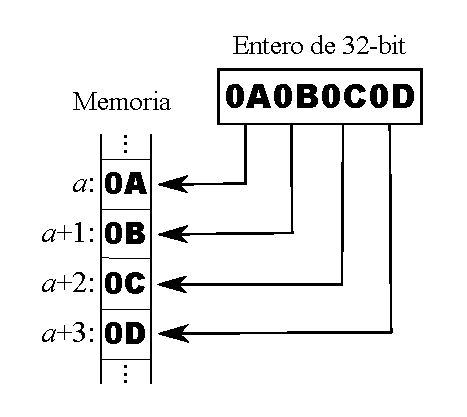
\includegraphics[width=\linewidth/3]{capitulo5/big_endian}
		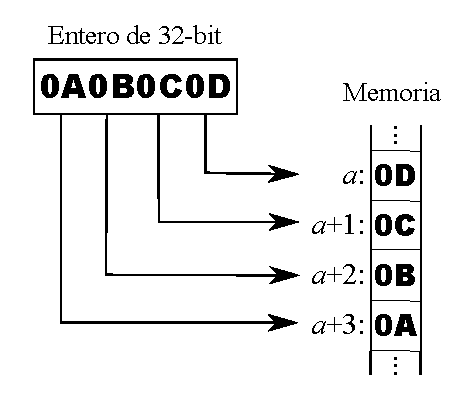
\includegraphics[width=\linewidth/3]{capitulo5/little_endian}
		\par\end{centering}
	\smallskip
	\caption[Big-endian y little-endian]{\label{fig:endianness} Big-endian (izquierda) y little-endian (derecha). \cite{wiki_endianness}}
\end{figure}
	
\smallskip

Por otro lado, también sabemos que ciertos valores, como el \textit{delta} de cada evento o el tamaño de datos de los meta-eventos, son de \textbf{longitud variable}: cada \textit{byte} tiene un significando de 7 \textit{bits}, los menos significativos. Mientras el último \textit{bit} sea 1, entonces el \textit{byte} siguiente del archivo corresponde, de igual forma, a otros 7 \textit{bits}, que se colocarían a la derecha (menos significativos).

\smallskip

\begin{figure}[H]
	\noindent \begin{centering}
		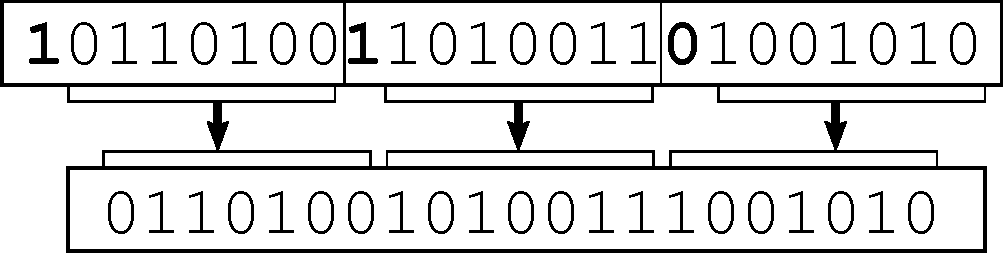
\includegraphics[width=\linewidth/2]{capitulo5/varlen}
		\par\end{centering}
	\smallskip
	\caption{\label{fig:varlen} Campo de longitud variable.}
\end{figure}

\smallskip

Además, podemos ver que todos los tipos de evento se numeran a partir de $80_{16}$, o sea, su \textit{bit} más significativo es 1. Si el analizador buscara un tipo de evento y encontrara un valor por debajo de este número, significa que el archivo está \textbf{obviando el tipo} de evento, y está indicando los parámetros ---cuyo tope es 127---.

\subsubsection{Prototipo}

En primer lugar hacemos una implementación sencilla en Python, que nos permita comprobar que hemos aplicado correctamente los conceptos.

Todos los valores de los tipos enumerados se hacen mediante constantes. Tal como dicta el diseño, la clase principal es \code{MidiFile}, que recibe un nombre de archivo. Los métodos se han implementado de la siguiente forma:

\begin{description}[style=nextline]
	\item[\code{\_\_init\_\_(self, pathname)}]
	Constructor: crea un archivo \acrshort{MIDI} completo desde un nombre de archivo (\code{pathname}). Abre el archivo, desempaqueta la cabecera y escribe los atributos del objeto en consecuencia. A continuación, inicializa la lista de pistas llamando al constructor de \code{MidiTrack} tantas veces como pistas indica el archivo.
	
	\item[\code{\_\_len\_\_(self)}]
	Devuelve el tamaño de la lista de pistas.
	
	\item[\code{\_\_getitem\_\_(self, key)}]
	Devuelve la pista indicada (\code{key}).
	
\end{description}

De esta forma, un archivo es sustancialmente una lista de pistas, y define los siguientes métodos:

\begin{description}[style=nextline]
	\item[\code{\_\_init\_\_(self, file)}]
	Constructor: crea una pista a partir de un fichero abierto (\code{file}), cuyo puntero debe estar al inicio de una nueva pista. Análogamente al constructor de \code{MidiFile}, analiza la cabecera, comprueba que sea válida y genera una lista de eventos utilizando para ello \code{MidiEvent.parseEvent()}
	
	\item[\code{\_\_iter\_\_(self)}]
	Permite iterar sobre los eventos la pista, devolviendo un iterador de la lista de eventos.	
\end{description}

Otra de las clases a implementar es \code{MidiEvent}, que representa cada uno de los eventos contenidos en un archivo, y contiene los siguientes métodos:

\begin{description}[style=nextline]
	\item[\code{\_\_init\_\_(self, delta, value, param1, param2)}]
	Constructor: crea un evento \acrshort{MIDI}, copiando en el sujeto (\code{self}) el retardo temporal (\code{delta}), el tipo de evento, junto al canal (\code{value}) y los parámetros (\code{param1} y \code{param2}).
	
	\item[\code{\_\_repr\_\_(self)}]
	Devuelve una cadena que expresa la representación del objeto, de la siguiente forma:
	
	\begin{center}
		<delta>: Event <tipo>@<canal> ( <Parámetro 1>, <Parámetro 2> )
	\end{center}
	
	\item[\code{note(self)}]
	Devuelve el código de nota (primer parámetro).
	
	\item[\code{velocity(self)}]
	Devuelve la intensidad sonora (primer parámetro).
	
	\item[\code{aftertouch(self)}]
	Devuelve la variación de intensidad, sita en el segundo parámetro si el tipo es \code{NOTE\_AFTERTOUCH} o en el primero en otro caso.
	
	\item[\code{controller(self)}]
	Devuelve el número de controlador (primer parámetro).
	
	\item[value\code{(self)}]
	Devuelve el valor del controlador (segundo parámetro).
	
	\item[program\code{(self)}]
	Devuelve el código de programa (primer parámetro).
	
	\item[pitch\code{(self)}]
	Devuelve el valor del \textit{pitch-bend} uniendo los parámetros:
	
	\begin{equation}
		pitch = p_1 \; | \; (p_2 << 7)
	\end{equation}
	
	\item[parseEvents(file)]
	Método de clase. Analiza todos los eventos de la pista actual en el archivo (\code{file}) hasta encontrar el meta-evento \code{END\_OF\_TRACK}. Su funcionamiento es el siguiente:
	
	\smallskip
	
	\begin{figure}[H]
		\noindent \begin{centering}
			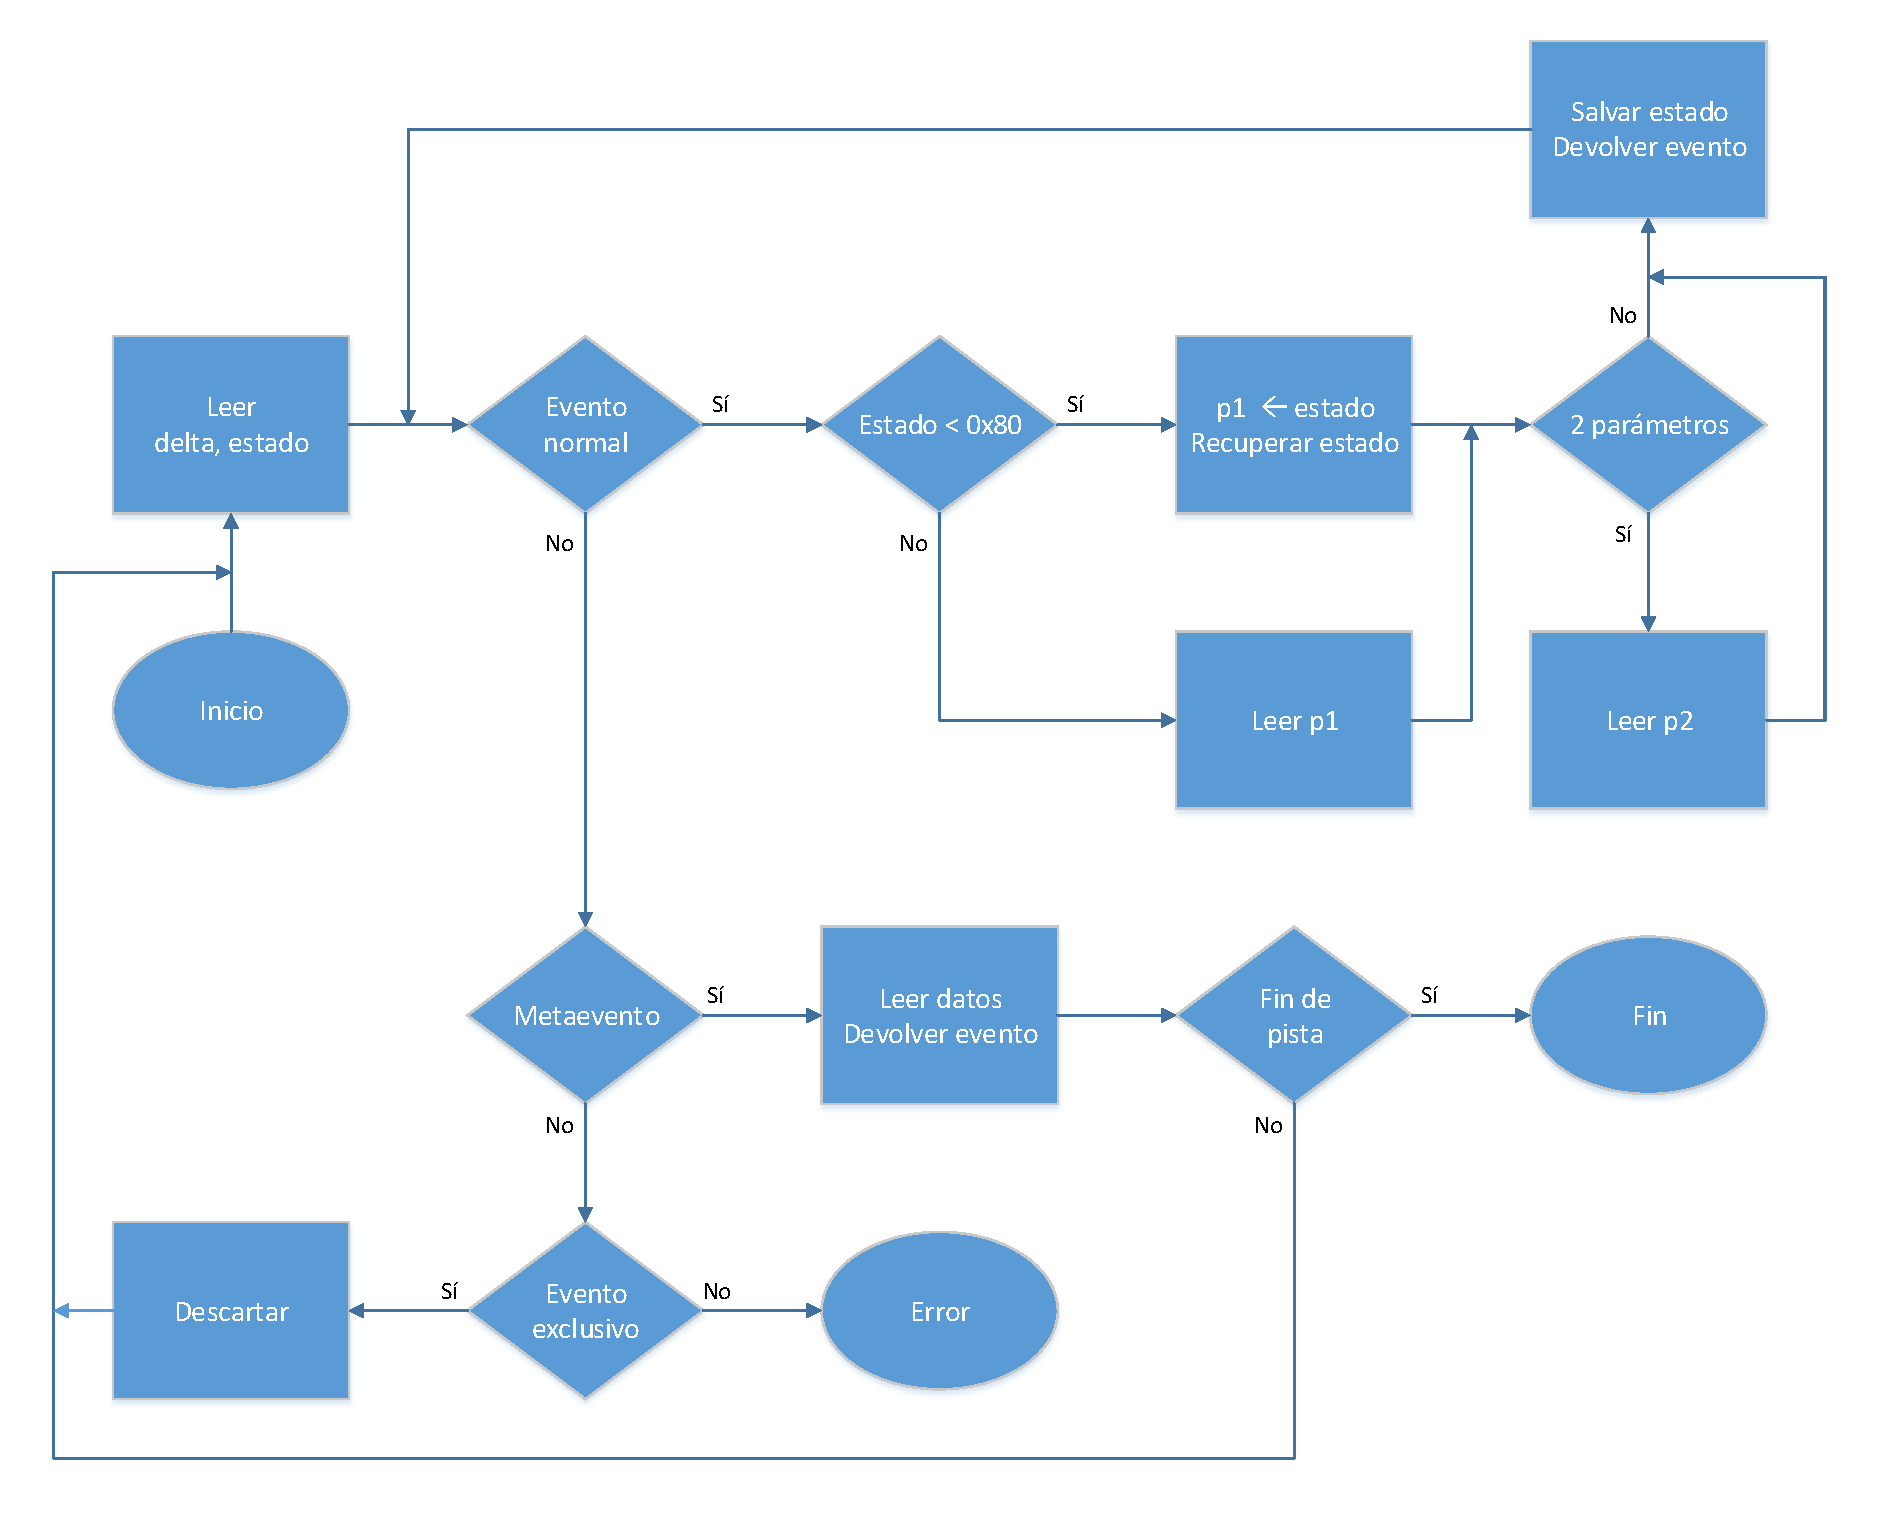
\includegraphics[width=\linewidth*2/3]{capitulo5/flujo_parser}
			\par\end{centering}
		\smallskip
		\caption{\label{fig:flujo_parser} Diagrama de flujo del analizador.}
	\end{figure}
	
	\smallskip
	
	\item[\code{varlen(file)}]
	Es una función auxiliar privada que recibe el archivo (\code{file}) apuntando a un campo de longitud variable (véase la figura \ref{fig:varlen}) y devuelve su valor.
	
\end{description}

Por último, la clase \code{MetaEvent} hereda de \code{MidiEvent} y, de acuerdo al diseño, tiene los siguientes métodos:

\begin{description}[style=nextline]
	\item[\code{\_\_init\_\_(self, delta, evtype, data)}]
	Constructor. Crea un metaevento copiando en el sujeto (\code{self}) el retardo temporal (\code{delta}), el tipo de meta-evento (\code{evtype}) y la cadena de datos (\code{data}).
	
	\item[\code{\_\_repr\_\_(self)}]
	Devuelve una cadena que expresa la representación del objeto, de la siguiente forma:
	
	\begin{center}
		<delta>: Meta-event <tipo>@<canal> ( <Parámetro 1>, <Parámetro 2> )
	\end{center}
	
	\item[\code{number(self)}]
	Devuelve el número de secuencia (primer \textit{byte} de la cadena).
	
	\item[\code{text(self)}]
	Devuelve la propia cadena de texto.
	
	\item[\code{channel(self)}]
	Devuelve el canal por defecto (primer \textit{byte} de la cadena).
	
	\item[\code{tempo(self)}]
	Calcula el \textit{tempo} en \textit{$\mu s / \quarternote$}. Este valor ocupa 3 \textit{bytes}, que se acuñan así:
	
	\begin{equation}
		(d_0 << 16) \; | \; (d_1 << 8) \; | \; d_2
	\end{equation}
	
	\item[\code{offset(self)}]
	Devuelve el desplazamiento temporal en una lista con el siguiente contenido:
	
	\begin{enumerate}
		\item Velocidad, según los 2 \textit{bits} más significativos del primer \textit{byte} de la cadena:
		
		\begin{itemize}
			\item $d_0[7:6] = 0 \Rightarrow 24 \; fps$
			\item $d_0[7:6] = 1 \Rightarrow 25 \; fps$
			\item $d_0[7:6] = 2 \Rightarrow 30 \; fps$
		\end{itemize}

		\item Número de horas ($d_0[5:0]$).
		\item Número de minutos ($d_1$).
		\item Número de segundos ($d_2$).
		\item Número de cuadros ($d_3$).
	\end{enumerate}

	\item[\code{time(self)}]
	Devuelve la marca de compás en una lista, de la siguiente forma:
	
	\begin{enumerate}
		\item Numerador: $d_0$.
		\item Denominador: $2^{d_1}$.
		\item Número de \textit{ticks} entre cada marca del metrónomo: $d_2$.
		\item Subdivisión, en \textit{fusas / click}: $d_3$.
	\end{enumerate}
	
	\item[\code{key(self)}]
	Devuelve la tonalidad en una lista, con los siguientes valores:
	
	\begin{enumerate}
		\item Número de $\sharp$ si es positivo, o número de $\flat$ si es negativo: $d_0$.
		\item Modo: $d_1$
	\end{enumerate}
\end{description}

Ya que es una prueba de concepto, el analizador emitirá un \textit{log} con  todos los datos extraídos de un archivo. Un ejemplo de salida es el siguiente:

\smallskip

\begin{figure}[H]
	\noindent \begin{centering}
		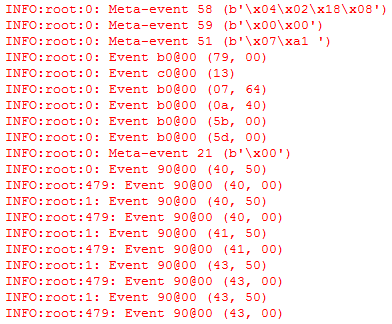
\includegraphics[width=\linewidth/2]{capitulo5/cap_parser}
		\par\end{centering}
	\smallskip
	\caption{\label{fig:cap_parser} Salida del prototipo del analizador.}
\end{figure}

\smallskip

\subsubsection{Implementación final}

Una vez puesto a prueba el analizador de \acrshort{MIDI} en Python, lo pasamos a C. Al ser un lenguaje no orientado a objetos, hay que introducir algunos cambios, pero el algoritmo es el mismo que el del prototipo. 

Sin embargo, las funciones no diferirán mucho del lenguaje anterior, porque en Python hay que poner el \textbf{sujeto} del método como primer parámetro, y en la nueva implementación haremos lo mismo. La diferencia más significativa es que tendremos que insertar un \textbf{destructor}.

En primer lugar, definimos los \textbf{tipos enumerados}:

\begin{description}
	\item[\code{enum format\_t}] Formato del archivo:
	
	\begin{description}
		\item[\code{SINGLE\_TRACK}] Una sola pista.
		\item[\code{MULTIPLE\_INDEPENDENT}] Varias pistas, simultáneas.
		\item[\code{MULTIPLE\_SIMULTANEOUS}] Varias pistas, independientes.
	\end{description}
	
	\item[\code{enum division\_t}] Unidad de medida de la división de tiempo:
	
	\begin{description}
		\item[TICKS\ PER\ BEAT] La división se especifica en \textit{ticks}/\quarternote.
		\item[FRAMES\_PER\_SECOND] La división se especifica en \textit{ticks/fotograma}.
	\end{description}
	
	\item[\code{enum midievent\_type\_t}] Tipo de evento \acrshort{MIDI}. Se enumeran en la tabla \ref{tab:midi_eventos}.
	\item[\code{enum metaevent\_type\_t}] Tipo de meta-evento. Se enumeran en la tabla \ref{tab:midi_metaeventos}.
	
	\item[\code{enum midimode\_t}] Modo tonal:
	
	\begin{description}
		\item[MAJOR] Modo mayor.
		\item[MINOR] Modo menor.
	\end{description}
\end{description}

Aparte del resto de transformaciones obvias, en pro de la velocidad de ejecución, hacemos los siguientes cambios:

\begin{enumerate}
	\item Anteponemos un \textbf{prefijo} a las funciones propias de cada estructura. El primer parámetro de todas ellas será un puntero a la misma.
	
	\item Eliminamos las funciones de consula que acceden llanamente a los parámetros, y a cambio sustituimos los parámetros simples por \textbf{uniones} con los nombres de las funciones.
	
	\item Ya que no podemos conocer a \textit{priori} el número de eventos que contendrá una pista, vamos a interpretar la composición propuesta por el diagrama \ref{fig:uml_midi} como una \textbf{lista enlazada} de eventos. Ya que la inserción y la lectura van a ser secuenciales, garantizamos una eficiencia algorítmica $O(1)$ en cada acceso.
\end{enumerate}

\subsection{Planificador}
\label{subsec:impl_planificador}

El planificador es la parte más crítica del sistema: debe cronometrar y ejecutar los eventos del archivo que está abierto, y atender a las llamadas declaradas en la interfaz.

El procedimiento básico es sencillo: cada evento tiene una marca de tiempo respecto al evento anterior. El sistema debe ''dormir'' el tiempo indicado ejecutar el evento, y avanzar al siguiente, hasta la marca de fin de pista.

Solo vamos a atender cuatro tipos de evento:

\begin{enumerate}
	\item Evento NOTE\_ON, para activar una nota.
	\item Evento NOTE\_OFF, para desactivar una nota.
	\item Metaevento TEMPO, para establecer la velocidad.
	\item Metaevento END\_OF\_TRACK, para terminar.
\end{enumerate}

\subsubsection{Prototipo}

De la misma forma que hicimos con el descodificador de archivos \acrshort{MIDI}, vamos a escribir un prototipo sencillo en Python. Recibirá un objeto de la clase \code{MidiFile} e interpretará una de sus pistas, a fin de estudiar la salida y hacer ajustes si es necesario.

El algoritmo se estructurará según el siguiente diagrama:

\smallskip

\begin{figure}[H]
	\noindent \begin{centering}
		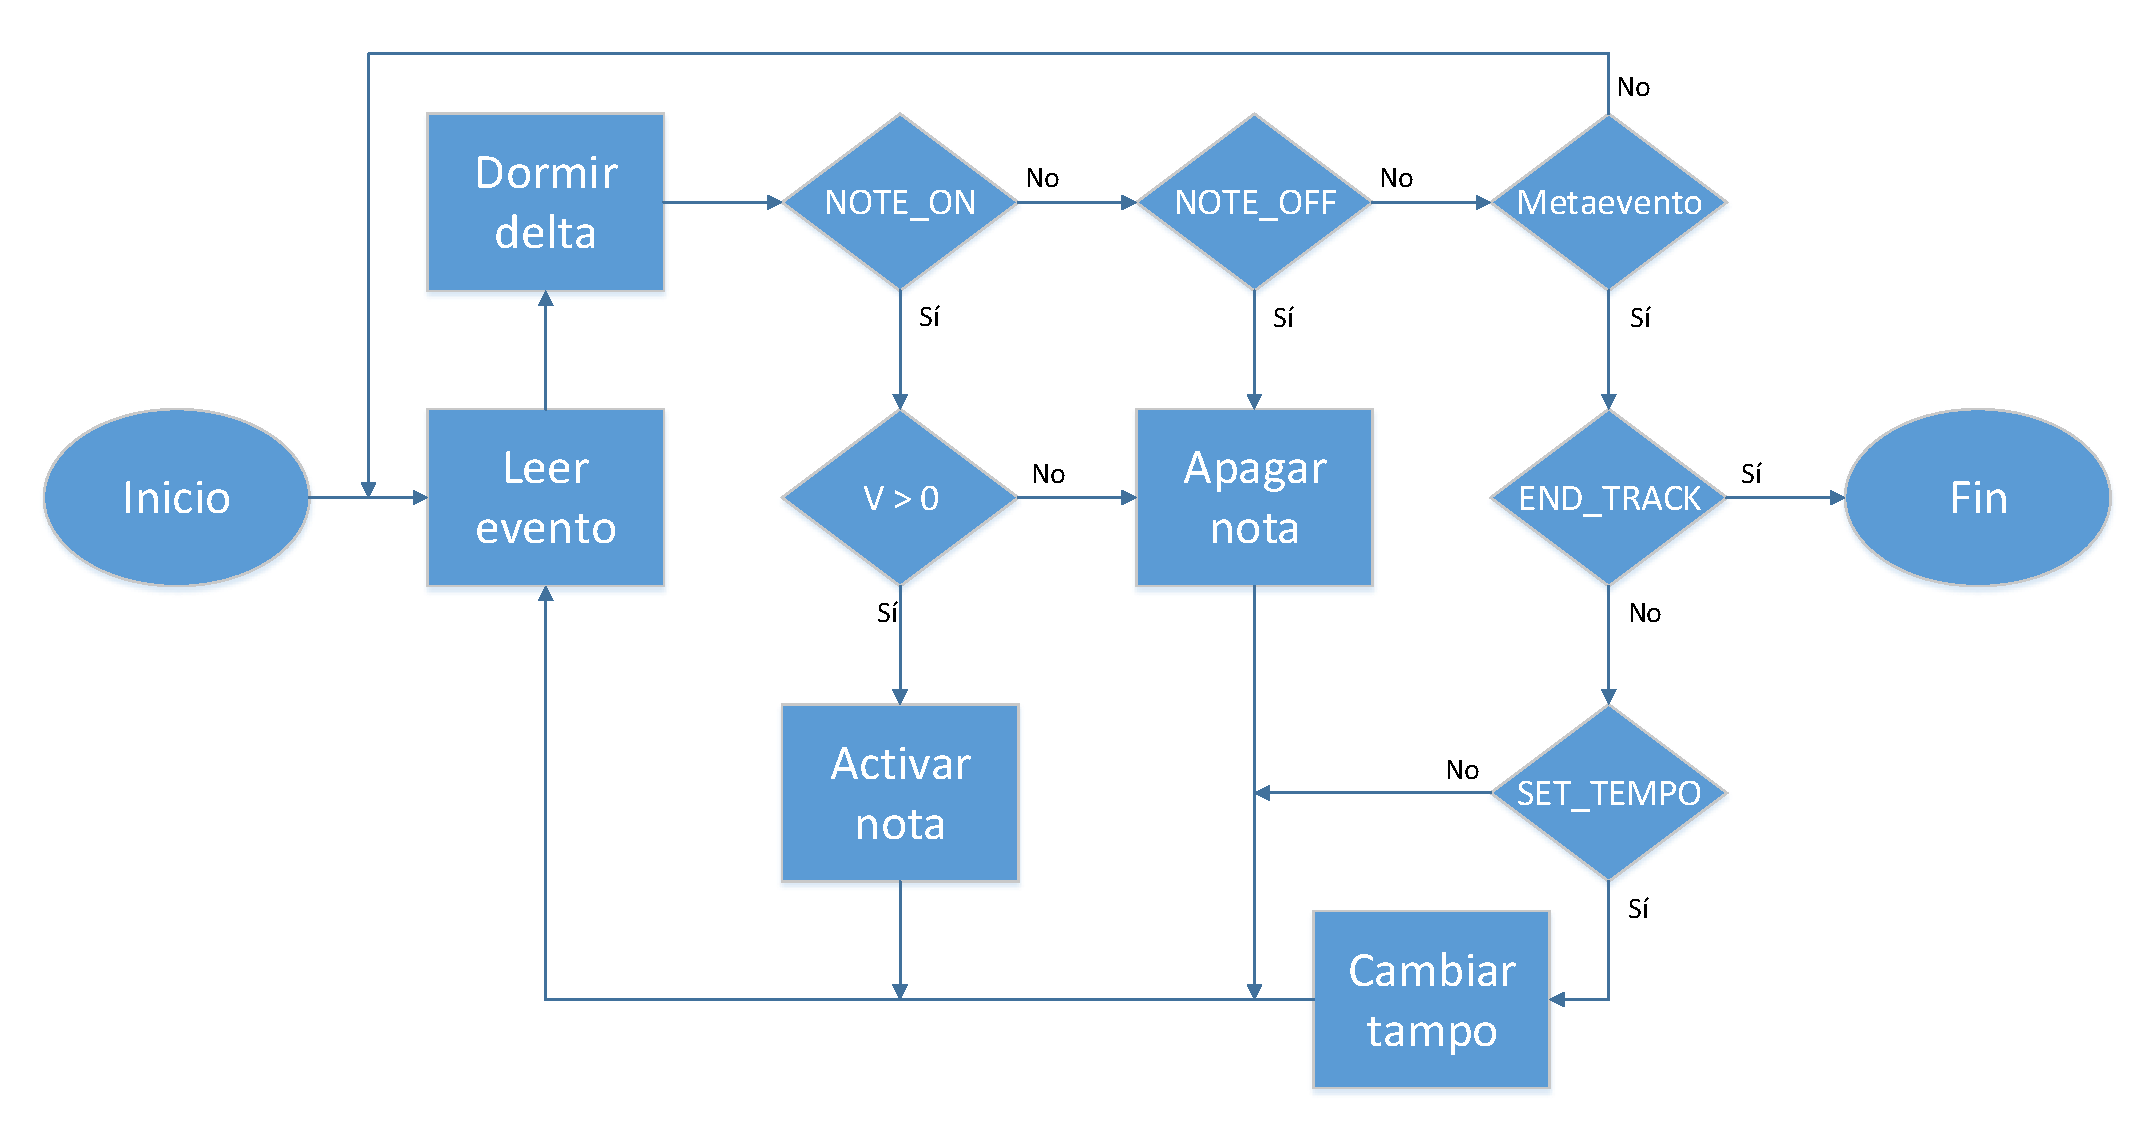
\includegraphics[width=\linewidth*3/4]{capitulo5/flujo_planificacion}
		\par\end{centering}
	\smallskip
	\caption{\label{fig:flujo_planificacion} Diagrama de flujo del planificador (simple).}
\end{figure}

\smallskip

En este caso, implementamos la clase \code{Instrument} para abstraernos de la configuración del instrumento, que tendrá que definir mínimamente algunas funciones de la interfaz de salida:

\begin{description}[style=nextline]
	\item[\code{state}]
	Estado del instrumento. Almacena qué notas están activas y cuáles inactivas. En lugar de una lista de \textit{booleanos}, será un simple número entero que trataremos como un campo de \textit{bits}, correspondiendo el más significativo a la nota más aguda, y el \textit{bit} menos significativo a la tecla más grave.
	
	\item[\code{length}]
	Especifica el número de notas que admite nuestro instrumento. Será el ancho del campo de \textit{bits}.
	
	\item[\code{offset}]
	Indica la primera nota del instrumento como el desplazamiento respecto a la primera nota \acrshort{MIDI}.
	
	\item[\code{\_\_init\_\_(self, length, offset}]
	Constructor. Crea las estructuras de datos en \code{self} conociendo la longitud del teclado (\code{length}) y la primera nota (\code{offset}).
	
	\item[\code{note\_on(self, note)}]
	Activa la nota indicada (\code{note}), comprobando antes si está dentro del rango cubierto por el teclado.
	
	\item[\code{note\_off(self, note)}]
	Apaga la nota indicada (\code{note}) si ésta pertenece al teclado.
	
	\item[\code{play(self, midi, track)}]
	Método del planificador. Cronometra y ejecuta la pista indicada (\code{track}) del archivo de la clase \code{MidiFile}. Esta función implementa el algoritmo que queremos prototipar.
	
\end{description}

La salida es muy simple: muestra para cada evento el cambio producido y el estado actual:

\smallskip

\begin{figure}[H]
	\noindent \begin{centering}
		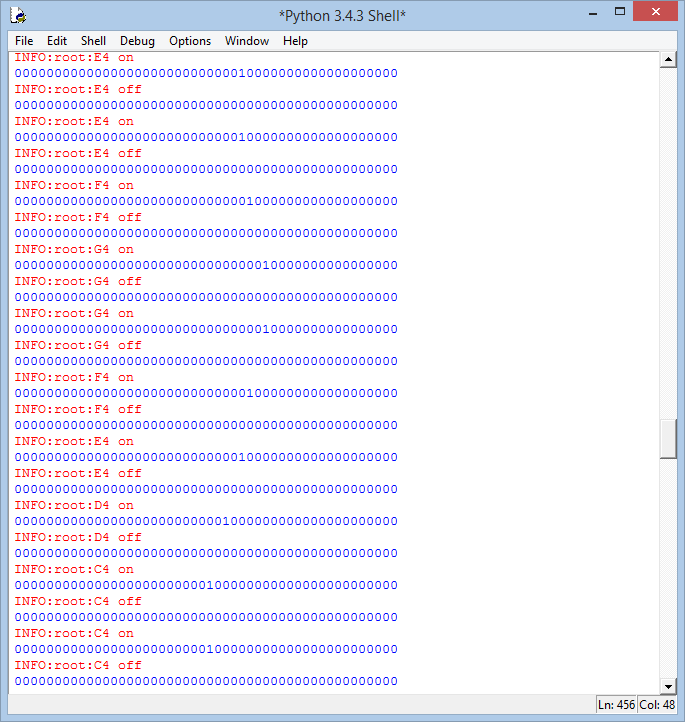
\includegraphics[width=\linewidth/2]{capitulo5/cap_pytest}
		\par\end{centering}
	\smallskip
	\caption{\label{fig:cap_pytest} Captura de pantalla del prototipo.}
\end{figure}

\smallskip

El prototipo nos sirvió para extraer dos objeciones:

\begin{enumerate}
	\item El \textbf{retraso} ($\Delta$) del evento es \textbf{inversamente proporcional} al \textit{tempo} y a la división de tiempo, indicada en la cabecera del archivo. Así pues, como el \textit{tempo} se expresa invertido, la espera se calcula de la siguiente forma:
	
	\begin{equation}
		retraso \; (\mu s)  = \frac{\Delta \; (ticks) \; \times \; tempo \; (\mu s / \quarternote)}{division \; (ticks / \quarternote)}
	\end{equation}
	
	\item La semántica para \textbf{desactivar una nota} no solo se hace con un evento NOTE\_OFF, sino que algunas piezas lo especifican con un evento NOTE\_ON con velocidad 0. Esto resulta útil para ahorrar espacio de almacenamiento, repitiendo el mismo tipo de evento.
\end{enumerate}

Una vez corregidos estos detalles, el prototipo cumple su objetivo correctamente. 

\subsubsection{Implementación final}

El paso siguiente es implantar el algoritmo en C con los correspondientes añadidos. El más importante es que, en realidad, no debemos ejecutar una pista, sino tantas como tenga el archivo. Tenemos dos alternativas:

\begin{enumerate}
	\item A \textbf{cada pista} se le asigna una \textbf{hebra} de ejecución. Se inician todas a la vez y se esperan al final.
	\item Ampliamos el algoritmo para que una sola hebra ejecute \textbf{todas las pistas} de forma \textbf{síncrona}.
\end{enumerate}

Como hemos podido deducir del diseño, nos decantamos por la \textbf{segunda opción}, considerando que todas las hebras tendrían que sincronizarse con la interfaz de salida, haciendo más llamadas de las necesarias. Además, las llamadas al sistema para retrasar la ejecución, así como las dedicadas a sincronizar la exclusión mutua, \textbf{desfasarían las pistas}, provocando una interpretación musical incorrecta.

Ya que el procesador del \textit{Raspberry Pi} solo tiene un \textbf{núcleo}, no vamos a ganar tiempo dividiendo el proceso en hebras, si sabemos manejar correctamente las pistas. Para ello, diseñamos el algoritmo descrito en la sección \ref{subsec:planificador}, que requerirá una sola hebra, que llamaremos \textbf{hebra de reproducción}.

El planificador define su interfaz de la siguiente manera:

\begin{description}[style=nextline]
	\item[enum player\_state\_t]
	
	Estado interno del reproductor.

	\begin{description}
		\item[\code{PAUSED}] En pausa.
		\item[\code{PLAYING}] Reproduciendo.
		\item[\code{STOPPED}] Detenido completamente.
		\item[\code{ENGINEER}] En modo Ingeniería. No se puede reproducir.
	\end{description}

	El orden de los tipos debe hacerse cuidadosamente para permitir al compilador generar un código óptimo \cite{vikman_switch}: Si las funciones utilizan la sentencia \code{switch} con etiquetas que comparten instrucciones (no todas acaban en \code{break}), es buena práctica que las etiquetas sigan el orden en que se ha declarado la enumeración.
	
	\item[\code{int player\_start(char **playlist, int n, int loop)}]
	Inicia la hebra de reproducción. Si ésta estaba en funcionamiento, primero la detiene. En primer lugar almacena la lista de rutas de archivo (\code{playlist}), el índice de la primera pieza a ejecutar (\code{n}) y la especificación de reproducir o no en bucle (\code{loop}).
	
	Ya que la terminación de la hebra anterior pudo ser natural o forzada, esta función es la encargada de eliminar la lista de reproducción precedente, si la hubiera. Una vez hecho esto, lanza la hebra de reproducción y devuelve el código de error (normalmente 0).
	
	\item[\code{int player\_wait()}]
	
	Bloquea a la hebra llamante hasta que la hebra de reproducción termine, y devuelve siempre \code{NULL}.
	
	\item[\code{int player\_pause()}]
	
	Comprueba que la hebra está funcionando y la pausa, cambiando el estado a \code{PAUSED}. A fin de evitar la espera activa de la hebra de reproducción, utilizaremos un semáforo de sincronización, que explicaremos más abajo.
	
	Devuelve 0 si ha pausado correctamente, o -1 si no estaba en ejecución.
	
	\item[\code{int player\_resume()}]
	
	Al contrario que la función anterior, comprueba que estaba en pausa, cambia el estado a \code{PLAYING} y señala el semáforo para despertar a la hebra de reproducción. Si estaba en reproducción, no hace nada. 
	
	Devuelve 0 si se ha reanudado la reproducción (o ya estaba funcionando), o -1 si estaba detenido.
	
	\item[\code{int player\_stop()}]
	
	Provoca la detención de la hebra de reproducción cambiando el estado a \code{STOPPED}, y espera a que la hebra termine efectivamente. Si estaba en pausa, primero despierta a la hebra para que termine por sí sola.
	
	Devuelve 0 si se ha detenido correctamente. Solo devuelve -1 si estaba en modo Ingeniería.
	
	\item[\code{player\_state\_t player\_state(char *file)}]
	
	Esta función devuelve el estado actual del reproductor. En caso de que estuviera en funcionamiento o pausado, copia en el parámetro \code{file} la ruta del archivo que está reproduciendo la hebra.
	
	\item[\code{int player\_engineer\_enter()}]
	
	Entra en el modo Ingeniería cambiando el estado a \code{ENGINEER}. Si la hebra estaba iniciada, previamente la detiene completamente. Si ya está en modo Ingeniería, no hace nada.
	
	Siempre devuelve 0.
	
	\item[\code{int player\_engineer\_exit()}]
	
	Sale del modo Ingeniería, si estaba dentro de él. El estado a la salida de \code{STOPPED}. Devuelve 0 si ha salido correctamente, o -1 si no estaba dentro.
\end{description}

Además, el módulo implementa los siguientes elementos de forma \textbf{estática}. Esto, en el ámbito del lenguaje C, significa que los símbolos no se exportan y, en consecuencia, solo las funciones dentro del módulo pueden llamarlas. Es el equivalente a los métodos privados en los lenguajes orientados a objetos. Son las siguientes:

\begin{description}[style=nextline]
	\item[\code{void* player\_run(void *arg)}]
	Punto de inicio de la hebra de reproducción. Consiste sencillamente en un bucle que recorre la lista de reproducción. En cada ciclo, abre el archivo correspondiente con ayuda del módulo \acrshort{MIDI} y lo ejecuta llamando a \code{playscore()}. Si la lectura falla, se ignora el archivo. En cualquier caso, después del uso, se destruye.
	
	Si se ha marcado la ejecución en bucle, al terminar de reproducir la lista, se vuelve al principio, indefinidamente. Si se diera el (improbable) caso de que todos los archivos de la lista fallen, la hebra termina.
	
	Devuelve siempre \code{NULL} como código de retorno del subproceso.
	
	\item[\code{int playscore(midifile\_t *file)}]
	
	Implementa el algoritmo de planificación para reproducir el archivo (\code{file}). Aplica el procedimiento descrito, al que añade una comprobación de estado en cada ciclo del bucle principal:
	
	\begin{description}
		\item[\code{PLAYING}] Continúa la ejecución normalmente.
		
		\item[\code{PAUSED}] Silencia la salida (manteniendo el estado) y pausa la reproducción. Como hemos adelantado, utiliza un semáforo para evitar la espera activa. El subproceso se bloquea hasta que otra hebra llame a \code{player\_pause()}, que es la que señala dicho semáforo.
		
		\item[\code{STOPPED}] Restablece la salida (borra el estado) y sale del bucle principal. 
	\end{description}
	
	Para un rendimiento óptimo, el bucle que ejecuta inmediatamente los eventos llama a \code{output\_noteon()} y \code{output\_noteoff()}, que cambian el estado del módulo de salida pero no la exportan efectivamente al instrumento. Cuando la racha termina, se sincroniza con la salida ---\code{output\_update()}--- y realiza la espera mediante una llamada a \code{nanosleep()}.

	El método de salida queda patente por el código de retorno:
	
	\begin{description}
		\item[0] Finalización natural.
		\item[1] Finalización forzada por una llamada a \code{player\_stop()}.
	\end{description}
	
\end{description}

\subsubsection{Metrónomo y velocidad}

Todas las partituras tienen una \textbf{marca de \textit{tempo}}, es decir, la velocidad a la que se reproducen. Esto se indica mediante el \textbf{meta-evento} correspondiente, habitualmente en la primera pista.

El planificador debe tener en cuenta este dato para reproducir correctamente la pieza. Si no se especificase el \textit{tempo}, se toma \textbf{por defecto} $\quarternote=120$, o $\quarternote=0.5 \;s$.

La interfaz de salida permite marcar \textbf{pulsos de metrónomo} para marcar el \textit{tempo} mediante un \acrshort{led} o un zumbador. Para controlar el tiempo, el planificador incorpora una \textbf{pista extra} compuesta por negras (\quarternote). Cuando se agota su \textit{delta}, en lugar de volcarlas a en la salida mediante \code{output\_noteon()}, las indica llamando a \code{output\_metronome()}.

\subsubsection{Concurrencia}

El planificador puede ser llamado por el servidor de \textit{socket}, el controlador del mando o el gestor del modo Ingeniería en cualquier momento, y en cualquier punto del reproductor. Esto puede llegar a generar \textbf{condiciones de carrera}, o incluso bloquear el sistema si dos módulos pretenden llevar a cabo acciones al mismo tiempo.

Además, debemos tener en cuenta posibles \textbf{usos ilegales} de la hebra de reproducción, como iniciarla, pausarla o detenerla varias veces consecutivas. Para evitar esto, como hemos descrito, las funciones públicas de control comprueban el estado antes de actuar.

A fin de no provocar una condición de carrera entre la hebra de reproducción y el resto, la primera nunca cambiará el estado, incluso si la partitura ha acabado. En su lugar activa una \textbf{variable ''bandera''} volátil (no afectada por optimizaciones del compilador) para ser leída por las funciones de control. Si está marcada, cambiarán automáticamente el estado a \code{STOPPED}.

Para evitar inconsistencias entre funciones públicas, todas ellas utilizarán un \textbf{\acrshort{mutex}} que monitoriza las llamadas, haciendo que toda función deba esperar a que termine cualquier otra que estuviera funcionando.

Por último, la \textbf{espera activa} se evita con un semáforo que se comporta como un \acrshort{mutex}: La función \code{player\_pause()} en primer lugar decrementa el semáforo y luego pone el estado a \code{PAUSED} para que, en la próxima vuelta, el planificador lo detecte y se bloquee esperando al semáforo. Cuando cualquier función quiera despertar al planificador, lo hace al revés: primero pone el estado a \code{PLAYING} y después desbloquea el semáforo, así el planificador no cae dos veces por error en el código de espera. Una vez el reproductor consigue el semáforo, lo vuelve a incrementar. 

Hacemos esto así para que el valor ''por defecto'' sea 1, evitando problemas si se diera el caso de solicitar una pausa justo cuando el planificador ha salido del bucle y no va a esperar al semáforo. La alternativa era utilizar un \acrshort{mutex}, pero no tenemos garantía de que lo vaya a desbloquear la misma hebra (e.g. si pausamos desde la interfaz gráfica, en una hebra, y reanudamos desde el mando, en otra). Un \acrshort{mutex} caería en una \textbf{condición indefinida}, mientras que un semáforo responde correctamente.

\subsection{Salida GPIO}

Esta parte del programa supone el \textbf{puente} entre el planificador y la \acrshort{PCB}, transformará instrucciones de activación y desactivación de notas en señales lógicas que emitiremos por el \acrshort{GPIO}. 

Este módulo se diseñó de forma muy flexible para que se pudiera adaptar fácilmente a cualquier órgano, o incluso se pudiera dirigir a otra interfaz, como tal vez la salida estándar ---de hecho, en el simulador de reproducción (sección \ref{subsec:simulador_reproduccion}) redefiniremos el funcionamiento para que así sea---.

Todas las implementaciones deben tener en común el hecho de almacenar el estado de todas las notas del instrumento. Las llamadas a \code{output\_noteon()} y \code{output\_noteoff()} cambiarán ese estado, y \code{output\_update()} volcará efectivamente esta información en la salida.

\subsubsection{Prototipo}

Inicialmente hicimos una \textbf{prueba de concepto} en Python para entender el funcionamiento de los registros de desplazamiento. Como ya explicamos en la sección de análisis (\ref{subsec:conexion_mecanica}), cada registro está dedicado a un componente del órgano, pero todos funcionan igual.

La idea es conseguir ver en los \acrshort{led}s la interpretación de una pieza conocida y fácilmente reconocible. Hemos tomado como \textbf{ejemplo} el famoso fragmento de la \textit{Oda a la alegría} de Ludwig van Beethoven:

\smallskip

\begin{figure}[H]
	\noindent \begin{centering}
		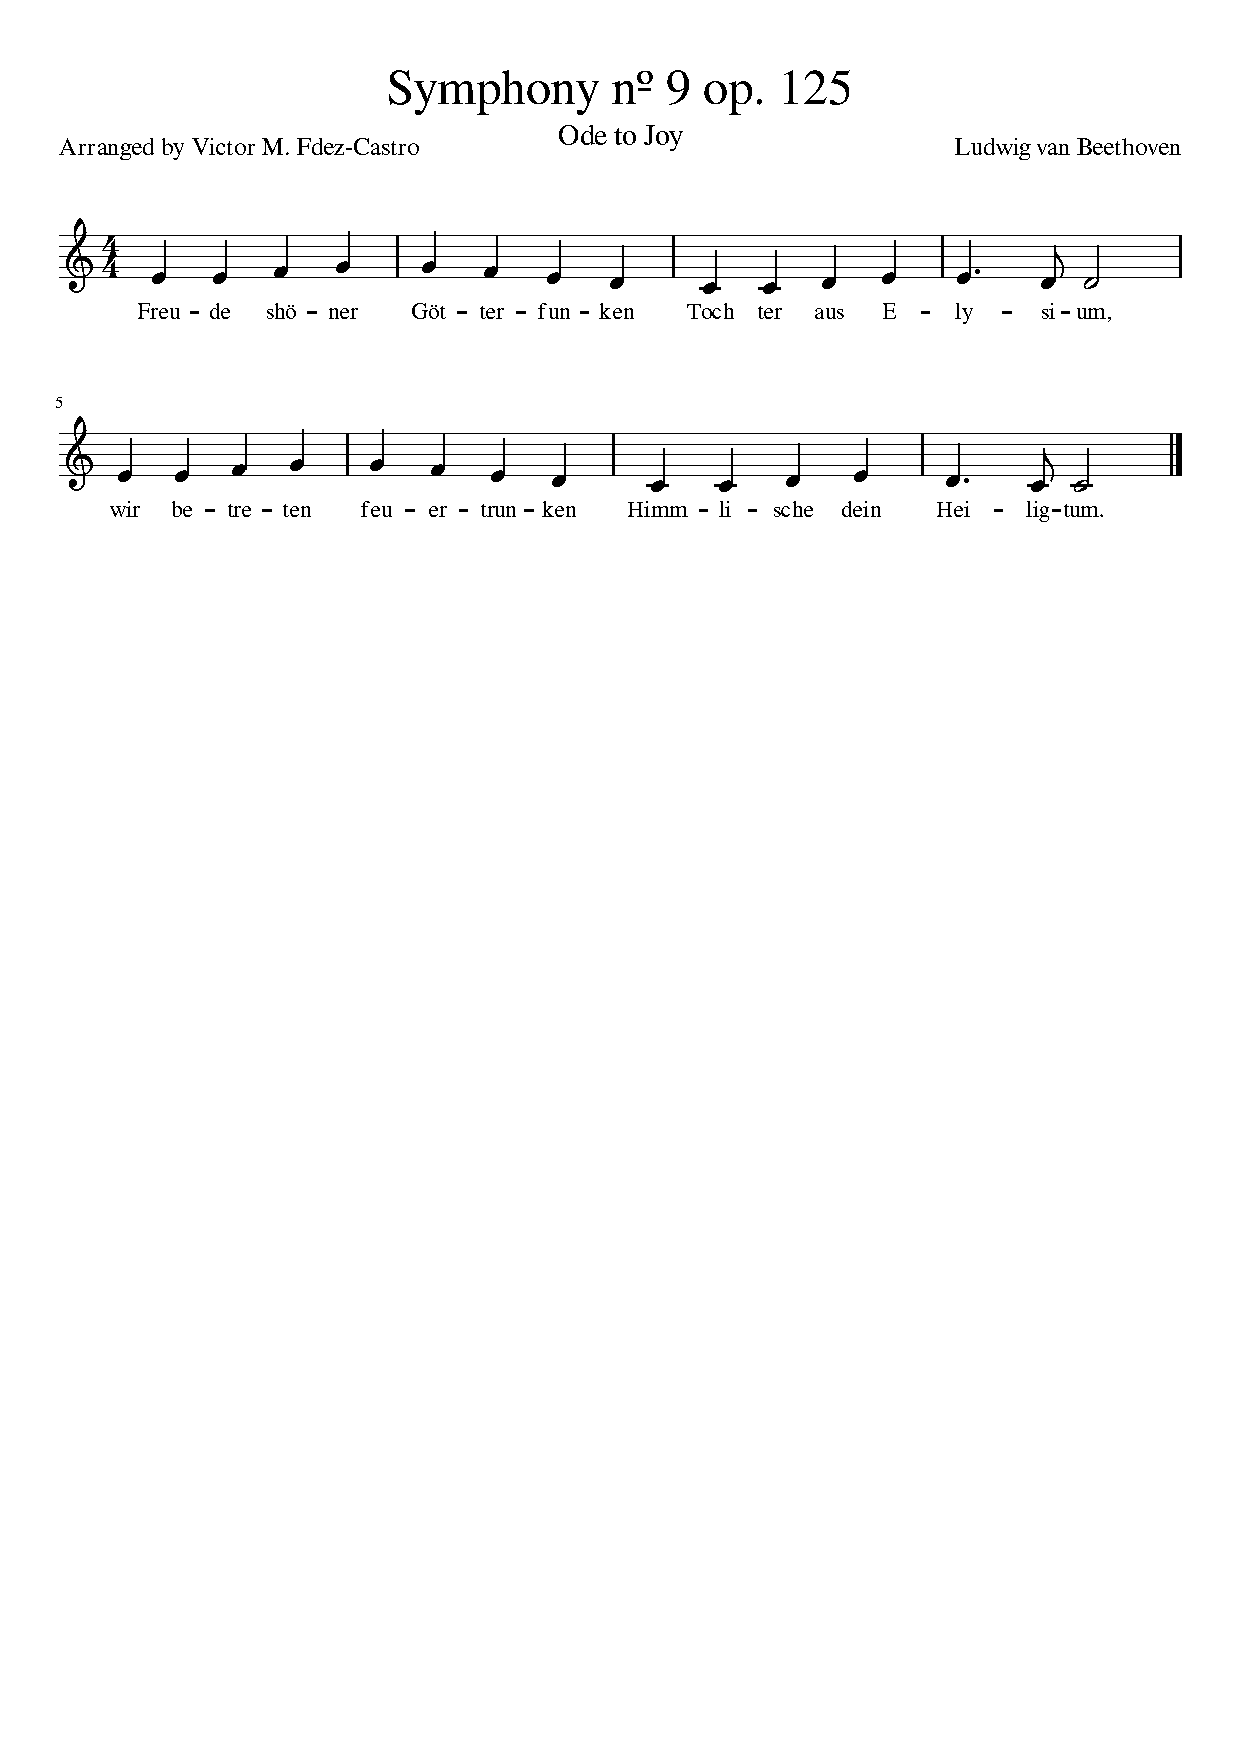
\includegraphics[clip=true,trim=20 580 20 30,width=\linewidth]{capitulo5/beethoven_1voz}
		\par\end{centering}
	\smallskip
	\caption{\label{fig:beethoven_1voz} Fragmento de la Oda a la Alegría de Beethoven.}
\end{figure}

\smallskip

Ya que no tenemos notas cromáticas, y disponemos de solo 7 \textit{bits} en la \acrshort{PCB}, vamos a establecer la siguiente equivalencia:

\smallskip

\begin{center}
	\begin{tabular}{|l|l|}
		\hline Do & \code{1000000} \\ 
		\hline Re & \code{0100000} \\ 
		\hline Mi & \code{0010000} \\ 
		\hline Fa & \code{0001000} \\
		\hline Sol & \code{0000100} \\
		\hline La & \code{0000010} \\
		\hline Si & \code{0000001} \\
		\hline 
	\end{tabular}
	\smallskip
	\captionof{table}{\label{tab:equiv_notas_prot} Equivalencia de notas en el prototipo.}
\end{center}

\smallskip

Cualquier \textbf{acorde} no sería más que una combinación de bits. Todo lo que tenemos que hacer es \textbf{volcar} cada nota por separado, \textbf{esperar} el tiempo que hagamos corresponder a una negra (\quarternote) y \textbf{silenciarlo} todo (volcar solo ceros). El procedimiento es muy sencillo:

\begin{enumerate}
	\item \textbf{Escribir} el valor de una celda del vector en el puerto \acrshort{GPIO} correspondiente.
	\item Emitir un \textbf{pulso} en el puerto conectado a SRCLK para \textbf{desplazar} y almacenar.
	\item Repetir los pasos 1 y 2 con el resto de \textit{bits}.
	\item Emitir un pulso en el puerto conectado a RCLK para \textbf{copiar} del registro de desplazamiento al registro de almacenamiento.
\end{enumerate}

Para emitir un pulso en el registro, actuamos de la siguiente forma, de acuerdo al manual técnico de los registros:

\begin{enumerate}
	\item Escribir ''1'' en el puerto llamando a \code{output()}.
	\item Esperar 100 \textit{ns} con una llamada a \code{sleep()}.
	\item Escribir ''0'' en el puerto.
\end{enumerate}

\subsubsection{Implementación final}

Este módulo va a ser llamado síncronamente por el planificador, por lo que todas las funciones que implementemos deben de ser tan rápidas como sea posible. El primer detalle importante es escoger una \textbf{estructura de datos} eficiente para almacenar el estado.

En este caso, todos los registros tienen el mismo tamaño, y conocemos de antemano las dimensiones, con lo cual, tenemos dos opciones. Teniendo en cuenta que hay que \textbf{indizar} por (nota, pista), vamos a deducir el número de operaciones necesarias para la escritura (aleatoria) y la lectura (secuencial):

\begin{enumerate}
	\item Una variable entera \textbf{como campo de \textit{bits}}.
	\begin{itemize}
		\item Cada \underline{escritura} requiere: indirección + multiplicación + suma + desplazamiento + conjunción + escritura. 
		\item Cada \underline{lectura} requiere: desplazamiento.
	\end{itemize}
	
	\item Una \textbf{matriz de \textit{bytes}}.
	
	\begin{itemize}
		\item Cada \underline{escritura} requiere: multiplicación + suma + escritura.
		\item Cada \underline{lectura} requiere: suma + indirección.
	\end{itemize}
\end{enumerate}

La matriz de \textit{bytes} está mejor \textbf{equilibrada}, sobre todo teniendo en cuenta que se va a hacer más escrituras que lecturas. El campo de \textit{bits}, además, nos limita a 32 \textit{bits} en total, lo que nos obligaría a hacer modificaciones cuando extendamos los registros.

Crearemos la matriz de esta manera:

\smallskip

\begin{center}
	\begin{tabular}{|c|cccc|}
		\hline & \multicolumn{4}{c|}{N pistas} \\
		\hline \multirow{7}{*}{\rotatebox[]{90}{M notas}} & $s_{0,0}$ & $s_{0,1}$ & $s_{0,2}$ & $s_{0,3}$ \\
		& $s_{1,0}$ & $s_{1,1}$ & $s_{1,2}$ & $s_{1,3}$ \\
		& $s_{2,0}$ & $s_{2,1}$ & $s_{2,2}$ & $s_{2,3}$ \\
		& $s_{3,0}$ & $s_{3,1}$ & $s_{3,2}$ & $s_{3,3}$ \\
		& $s_{4,0}$ & $s_{4,1}$ & $s_{4,2}$ & $s_{4,3}$ \\
		& $s_{5,0}$ & $s_{5,1}$ & $s_{5,2}$ & $s_{5,3}$ \\
		& $s_{6,0}$ & $s_{6,1}$ & $s_{6,2}$ & $s_{6,3}$ \\
		\hline 
	\end{tabular}
	\smallskip
	\captionof{table}{\label{tab:matriz_estatica} Configuración de las notas en el estado.}
\end{center}

\smallskip

El compilador, conociendo las dimensiones, convertirá la matriz estática en un \textit{array} de la siguiente forma:

\smallskip

\begin{center}
	\begin{tabular}{|c|}
		\hline $M\times N$ \textit{bytes} \\
		\hline $s_{0,0}$ $s_{0,1}$ $s_{0,2}$ $s_{0,3}$ $s_{1,0}$ $s_{1,1}$ ... $s_{6,2}$  $s_{6,3}$ \\
		\hline 
	\end{tabular}
	\smallskip
	\captionof{table}{\label{tab:matriz_fisica} Disposición física de la matriz en memoria.}
\end{center}

\smallskip

Con esta estructura, el acceso aleatorio para escribir un valor en el estado se hará con la siguiente fórmula:

\begin{center}
	$s_{nota,pista} = v_{nota \times N + pista}$
\end{center}

Para \textbf{volcar} la información en los registros, seguiremos los mismos pasos que en el prototipo, pero en lugar de transmitir a un puerto \acrshort{GPIO}, transmitiremos a tantos como pistas tengamos, antes de enviar el pulso a SRCLK, que desplaza las notas de todos los registros a la vez.

Hemos organizado la matriz para que la lectura se hagan en el \textbf{orden estricto} en que están los datos en memoria, con lo cual, en lugar de acceder a la matriz directamente y obligar al compilador a hacer una multiplicación y una suma, utilizaremos \textbf{aritmética de punteros} para movernos por ella.

\subsection{Metrónomo}

A diferencia de las notas musicales, el metrónomo \textbf{no se almacena} en el estado ni se retrasa su ejecución hasta llamar a \code{output\_update()}, sino que debe marcarse tan rápido como se ejecute la función \code{output\_metronome()}

Para hacer sonar los pulsos de metrónomo, la \acrshort{PCB} cuenta con un zumbador, tal como se definió en la fase de análisis. A pesar de que está diseñado para emitir sonidos agudos continuados, vamos a generar un \textbf{pulso de 1 \textit{ms}}.

Para obtener la mayor velocidad de respuesta sin retrasar al planificador, la función \code{output\_init()} crea una \textbf{hebra} que espera un \textbf{semáforo}. \code{output\_init()} se limita a enviar una señal a dicho semáforo para despertar a la hebra y hacerla enviar un pulso al zumbador.

\subsubsection{Acceso directo al GPIO}

La siguiente cuestión es cómo acceder al \acrshort{GPIO}. Conocemos bien el \textbf{sistema de archivos} especial que nos brinda Linux, pero el hecho de actuar por medio de llamadas al sistema y acceso a ficheros para algo tan elemental podría resultar \textbf{ineficiente}.

Los puertos \acrshort{GPIO} son \textbf{pines físicos} del \acrshort{SOCA}, y se puede acceder a ellos mediante el periférico correspondiente mediante \textbf{acceso a memoria}. Estudiando el manual del BCM2835, obtenemos la siguiente información:

\smallskip

\begin{center}
	\begin{tabular}{|l|l|}
		\hline 0x20200000 & Dirección base \\
		\hline
		\hline Base + 0 & \multirow{6}{*}{Selección de función} \\
		\cline{1-1} Base + 4 & \\
		\cline{1-1} Base + 8 & \\
		\cline{1-1} Base + 12 & \\
		\cline{1-1} Base + 16 & \\
		\cline{1-1} Base + 20 & \\
		\hline Base + 24 & Reservado \\
		\hline Base + 28 & \multirow{2}{*}{Poner a ''1''} \\
		\cline{1-1} Base + 32 & \\
		\hline Base + 36 & Reservado \\
		\hline Base + 40 & \multirow{2}{*}{Poner a ''0''} \\
		\cline{1-1} Base + 44 & \\
		\hline \multicolumn{2}{|c|}{...} \\
		\hline 
	\end{tabular}
	\smallskip
	\captionof{table}{\label{tab:gpio_struct} Direcciones físicas del GPIO.}
\end{center}

\smallskip

El controlador de \acrshort{GPIO} utiiza registros de 32-\textit{bit}. Para obtener un puntero a una dirección de memoria física, tan solo necesitamos hacer una llamada a \code{mmap(file = ''dev/mem'', offset = 0x20200000)} \cite{soii}. 

A partir de ahí, podemos acceder a cada registro con los \textbf{desplazamientos} adecuados. Hay un \textbf{banco} de registros para poner a ''1'', escribiendo un 1 lógico en el \textit{bit} correspondiente al número de puerto, y otro para poner a ''0'', escribiendo un 1 lógico en el \textit{bit} adecuado.

De esta forma logramos la mayor \textbf{eficiencia}, tanto por el acceso directo a memoria como la posibilidad de escribir en todas las pistas más el reloj en \textbf{una sola operación} de escritura.

\subsubsection{Mapeo y tolerancia}

Huelga decir que para logar una óptima reproducción, será necesario adaptar las partituras al órgano en cuestión, ya que cada ejemplar tendrá una rango de notas y un conjunto de registros distintos. Nuestra aplicación será lo más \textbf{estándar} posible a la hora de leer un archivo \acrshort{MIDI}, por ello, y para \textbf{evitar errores} por incompatibilidad, debemos contemplar que podemos recibir un archivo \acrshort{MIDI} cualquiera.

El número de pistas y el tamaño de cada una es conocido en tiempo de \textbf{compilación}, como ya sabemos. Las funciones \code{output\_noteon()} y \code{output\_noteoff()} reciben el código de nota y el índice de pista, que se escribirá en el estado. Un detalle simple, pero importante, será \textbf{descartar} cualquier nota fuera del rango, y cualquier pista no declarada.

Por otro lado, no es estrictamente necesario que el orden de las pistas en el archivo (pentagramas) coincida con el orden de los registros en la \acrshort{PCB}. Para modelar esto, tendremos un \textbf{\textit{array}} con los números de puerto \acrshort{GPIO} asociados a cada pista del archivo \acrshort{MIDI}:

La \textbf{asignación por defecto}, para el órgano de prueba, será la siguiente:

\smallskip

\begin{center}
	\begin{tabular}{|l|c|c|c|c|}
		\hline \textbf{Pista} & 1 & 2 & 3 & 4 \\
		\hline \textbf{Puerto GPIO} & 02 & 03 & 17 & 04 \\
		\hline \textbf{Canal PCB} & S1 & S2 & S4 & S3 \\
		\hline \textbf{Componente} & Teclado 1 & Teclado 2 & Registros & Pedalier \\
		\hline 
	\end{tabular}
	\smallskip
	\captionof{table}{\label{tab:asig_canales} Asignación de pistas al GPIO.}
\end{center}

\smallskip

\subsection{Servidor socket}

Esta parte del programa es la vía de acceso al servicio, se dedica a atender las peticiones de otras aplicaciones, como la interfaz web, según el protocolo de comunicación diseñado. Para ello utiliza un \textit{socket} de Unix \cite{wiki_socket}, similar a los \textit{sockets} de Internet, pero dedicado a la comunicación inter-proceso dentro de la misma máquina, a través de memoria compartida.

El \textbf{código de inicialización}, en la función \code{socket\_init(uid, gid)}, hace lo siguiente:

\begin{enumerate}
	\item Crea la estructura de archivos de programación.
	\item Asigna un archivo \textit{socket} en el sistema de archivos. Por defecto será \code{/run/organd.sock}.
	\item Prepara el zócalo para escucha (modo servidor).
	\item Establece como propietario el \acrshort{UID} y el \acrshort{GID} que recibe como parámetros, correspondientes a un usuario especial.
	\item Solicita ignorar la señal \code{SIGPIPE}, que colgaría el programa si un cliente se desconecta repentinamente.
\end{enumerate}

Por otro lado, el procedimiento \code{socket\_loop()} inicia el \textbf{bucle de escucha}: se bloquea hasta recibir una nueva petición y, a partir de ahí, actúa siguiendo el protocolo establecido en la sección \ref{sec:protocolo}, transmitiendo las órdenes al planificador.

Recordemos que el planificador recibe una lista de nombres de archivo, como una \textbf{matriz de caracteres}, de cuya destrucción se ocupa él mismo. La función \code{socket\_play()} pues, \textbf{clasifica} la lista de archivos recibidas en la cadena a una lista de cadenas, antes de pasarla al planificador (\code{player\_start()}).

\subsection{Servidor UART}

El módulo de servicio del \acrshort{UART} tiene una estructura similar al del \textit{socket}, solo que atiende a las peticiones del mando a distancia que llegan por el \textbf{puerto en serie}. Por un lado el protocolo de comunicación es más sencillo, por otro, no conocemos la información de las listas asociadas a un botón, por lo que hay que hacer consultas a la \textbf{base de datos}.

En primer lugar, \code{uart\_init()} abre la comunicación con el puerto en serie y establece los \textbf{parámetros de configuración} adecuados al receptor del mando (9600 \textit{baudios}) y bloqueo hasta recibir 10 caracteres, que es la longitud de la cadena que esperamos recibir.

Para iniciar el \textbf{bucle de recepción} implementamos \code{uart\_loop()}, que simplemente crea una hebra y la inicia en \code{uart\_run()}. Como adelantamos en la fase de análisis (sección \ref{analisis_mando}), el descodificador envía en primer lugar el \textbf{número de serie} del mando, que comparamos con el número de serie registrado en tiempo de compilación. 

A continuación leemos el \textbf{código del botón}, codificado como ya describimos, y seguimos adelante según este esquema para un mando de dos botones:

\begin{description}
	\item[Botón 1] Inicia la lista de reproducción asignada al botón 1.
	\item[Botón 2] Reproduce la lista asignada al botón 2.
	\item[Ambos] Pausa la reproducción, o la reanuda.
\end{description}

Para reproducir una lista, escribimos el código en una función auxiliar, \code{uart\_playlist()}, que se comunica con la \textbf{base de datos} en busca de una lista de reproducción asignada, y los nombres de archivo correspondientes, para generar un \textit{array} de rutas de fichero y llamar a \code{player\_start()}.

Por otro lado, la función de \textbf{pausa/reanudar} llama a la función \code{uart\_pause()}, encargada de consultar el estado del planificador y actuar en consecuencia: si estaba funcionando llama a \code{player\_pause()}, y si estaba pausado ejecuta \code{player\_resume()}; en otro caso no realiza ninguna acción.

La función para \textbf{detener} está implementada aunque actualmente no se utiliza. Simplemente hace llamar a \code{player\_stop()}, cuyo funcionamiento es inocuo si el reproductor ya estaba parado.

\subsection{Comunicación con la base de datos}

El módulo receptor del mando necesita conocer la asignación de botones a listas, y las rutas de archivo de las partituras pertenecientes a las listas. Esta información está almacenada en una base de datos, y el acceso se hace a través de un módulo aparte, con objeto de presentar una interfaz independiente del \acrshort{SGBD} que utilicemos.

Como explicaremos más adelante, utilizaremos \textbf{MySQL}, de forma que nuestro módulo utilizará la biblioteca cliente de MySQL para C. Así, la implementación de las funciones de inicio y cierre, \code{db\_init()} y \code{db\_destroy()}, respectivamente, simplemente abren la comunicación con MySQL mediante \code{mysql\_real\_connect()} y la terminan con \code{mysql\_close()}.

Para conectarse a la base de datos hay que conocer el \textbf{nombre de usuario} y la \textbf{contraseña} asignados a dicha base, que conocemos de antemano y están guardados en tiempo de compilación.

La última función diseñada, \code{db\_query()}, es la encargada de \textbf{consultar} la lista de archivos en la base de datos, conocido el número de botón pulsado. La información recibida es devuelta como un puntero a una matriz de caracteres, a tratar por el módulo llamador.

\subsection{Modo Ingeniería}

El diseño ha contemplado un control de la mecánica del sistema, a través del \acrshort{LCD} y el codificador rotatorio, que consiste en un menú que permite entrar en modo Ingeniería para \textbf{activar y desactivar las notas} a placer, de una en una. De la misma forma, tendremos la opción para activar y desactivar el \textbf{metrónomo}, así como \textbf{apagar y reiniciar} el sistema.

Como especificamos en la sección \ref{subsec:ingenieria}, la gestión de esta interfaz está diseñada como una \textbf{máquina de estados}. La función \code{periph\_init()} se encarga de preparar los puertos \acrshort{GPIO} asignados al codificador, e inicializa el \acrshort{LCD}. Por seguridad, activaremos la polarización de los puertos \acrshort{GPIO} de acuerdo a la utilizada por el codificador:

\begin{itemize}
	\item \textit{Pull-up} para los canales A y B (giro).
	\item \textit{Pull-down} para el pulsador.
\end{itemize}

Por último, esta función crea una \textbf{hebra independiente} para gestionar la máquina de estados.

\subsubsection{Control de entrada}

El codificador rotatorio producirá los eventos de entrada. De acuerdo con el análisis de este dispositivo (sección \ref{subsec:rotary}), entre dos puntos de equilibrio cambia el canal A, y entonces, dependiendo del valor de los canales A y B ---si coinciden o difieren--- interpretaremos un giro a la izquierda y otro a la derecha.

De esta forma, tenemos que esperar dos eventos:

\begin{enumerate}
	\item Cambio en el canal A.
	\item Subida en el pulsador.
\end{enumerate}
	
A fin de evitar la \textbf{espera activa}, se crearán dos hebras que se bloquearán hasta recibir la señal correspondiente, cuando llamarán a dos funciones asignadas como \textit{callbacks}:

\begin{description}[style=nextline]
	\item[rot\_change()] Ha cambiado el canal A. Lee A y B, los compara y activa la bandera correspondiente.
	\item[rot\_push()] Se ha pulsado el botón. Solicita una espera de 1 \textit{ms} y activa la bandera de pulsación.
\end{description}

Ambas funciones utilizan un \textit{array} de banderas (\textit{flags}) para indicar qué evento está pendiente de atender, y señalan un \textbf{semáforo} para el control de la máquina de estados.

La pulsación está sujeta a problemas de \textbf{rebotes}, que podrían disparar la función varias veces aun pulsando el botón una vez. Como vimos en la figura \ref{fig:rebotes}, existe una \textbf{incertidumbre} de $118 \; \mu s$ desde que comienza a subir la señal hasta que se queda estable. Por seguridad, estableceremos un tiempo de 1 \textit{ms} antes de hacer una \textbf{segunda lectura}, si sigue siendo positiva, aceptamos la pulsación.

\subsubsection{Máquina de estados}

La función principal de la hebra de control es \code{periph\_run()}, que implementa un bucle para atender los eventos y definir el \textbf{estado siguiente}. La implementación de esta función sigue la especificación del diagrama de la figura \ref{fig:engineer}.

Cuando entra en modo Ingeniería, llama a la función \code{player\_engineer\_enter()} del planificador, que lo \textbf{aísla de la salida} del \acrshort{GPIO}, dejándolo libre para actuar sobre él con las llamadas a bajo nivel \code{output\_noteon()} y \code{output\_noteoff()}.

Por otro lado, el menú ofrece la opción de activar y desactivar el \textbf{metrónomo}, para ello hace uso de las función \code{output\_metronome\_enable()}. Además, existe otro menú para \textbf{controlar la energía} del sistema, esto se hace llamando a la orden \code{shutdown} con la función \code{system()}.

Al final del bucle, el subproceso se bloquea esperando que el usuario actúe y el \textit{callback} correspondiente señale el semáforo.

\subsubsection{Control de salida}

La salida de este módulo se hace sobre el \acrshort{LCD}, que realimentará las acciones del usuario en modo Ingniería. Sin embargo, mientras no se use este modo, se mostrará el \textbf{estado del planificador} y, en su caso, la ruta del \textbf{archivo} que se está reproduciendo.

Para ello, cuando el bucle de la máquina de estados ha calculado el estado siguiente, se refresca la pantalla en función del nuevo estado, ya sea:

\begin{enumerate}
	\item Navegar por el menú.
	\item Mostrar el estado del reproductor.
	\item En modo Ingeniería, indicar la pista actual y la nota que está activa.
\end{enumerate}

Para mostrar el estado del reproductor, hay que tener en cuenta que la información va a cambiar aunque el usuario no interactúe con los mandos. Por ello, la espera del semáforo será \textbf{temporizada}: si tras un tiempo determinado el usuario no toca el control, la hebra se despierta sola y refresca la pantalla.

\subsection{Inicio del demonio}

Ahora vamos a crear el punto de inicio de nuestro servicio, para que se inicie durante el arranque del sistema operativo del \textit{Raspberry Pi}. Lo que este módulo hará será muy sencillo: iniciar todos los módulos y llamar a los bucles de escucha que incorporan en hebras diferentes.

\subsubsection{Características}

Un demonio ---en nomenclatura de la familia Unix--- es un programa que se ejecuta en segundo plano, es iniciado por el \textbf{\textit{boostrap}} del sistema operativo y no interactúa directamente con el usuario. Está diseñado para dar servicio a otras aplicaciones. Ni siquiera utiliza la entrada y salida estándar, en su lugar usa el registro del sistema.

Al mismo tiempo, y paradójicamente, debe \textbf{terminar} lo antes posible para permitir que continúe el arranque del sistema. Para iniciar correctamente el demonio, la función principal del programa hará lo siguiente: \cite{shahmir_daemon}

\begin{enumerate}
	\item Crea una copia de sí mismo mediante una bifurcación, llamando a \code{fork()}. Como ya sabemos, esta función devuelve el ID del hijo al proceso padre y 0 al proceso hijo. En este punto, el padre termina.
	
	\item Crea una nueva sesión mediante \code{setsid()}, convirtiendo al proceso hijo en líder de su grupo de procesos.
	
	\item Cambia la carpeta de trabajo por la raíz del sistema, llamando a \code{chdir(''/'')}.
	
	\item Cierra mediante \code{close()} los descriptores de archivo de la entrada y salida estándar: \textit{stdin}, \textit{stdout} y \textit{stderr}.
	
	\item Abre el \textit{log} del sistema con \code{openlog()}.
	
	\item Inicia el módulo del \textit{socket}.
	
	\item Arranca el módulo del mando a distancia.
	
	\item Inicia el módulo del modo Ingeniería.
	
	\item Rebaja sus permisos a los del \acrshort{UID} y el \acrshort{GID} recibidos.
	
	\item Inicia el bucle de escucha del servidor del puerto en serie (en otra hebra).
	
	\item Llama al bucle de servicio del \textit{socket}.
	
\end{enumerate}

Otra acción importante es \textbf{programar el cierre} controlado mediante una sencilla función que detenga la reproducción y llame a las funciones de limpieza ---las que terminan en \code{\_destroy()}---:

\begin{enumerate}
	\item Planificar dicha llamada cuando se termine el programa, haciendo uso de \code{atexit}.
	\item Programar una salida normal ---\code{exit(0)}--- cuando se reciba la señal SIGTERM, que es la que envía por defecto \code{kill} y la que corresponde a pulsar Ctrl+C.
\end{enumerate}

\subsubsection{Script de arranque}

Conforme a la base estándar de Linux ---\acrshort{LSB}, \textit{\acrlong{LSB}}---, el arranque del sistema buscará un \textit{script} para iniciar el demonio en una ubicación dependiente del nivel de ejecución, y lo llamará con el argumento \code{''start''}. \cite{debian_lsbinit}

Con objeto de arrancar los distintos servicios en el orden correcto para preservar dependencias, debemos escribir una \textbf{cabecera} en el código, que utilizará la orden \code{insserv} para registrar el servicio. En ella especificaremos la siguiente información:

\begin{enumerate}
	\item Requiere el servicio \code{syslog}, para el \textit{log} del sistema.
	\item Se iniciará en los niveles de ejecución 2, 3, 4, 5 (multiusuario). \cite{wiki_runlevel}
	\item Se parará en los niveles 0, 1 y 6 (monousuario, apagar y reiniciar).
\end{enumerate}

De acuerdo al estándar, el \textit{script} atenderá a las siguientes órdenes:

\begin{description}
	\item[start] Arranca el demonio. Busca el proceso con \code{ps -e | grep}, si no lo encuentra, consulta el \acrshort{UID} y \acrshort{GID} del usuario dedicado, y llama al servicio pasando ambos argumentos.
	
	\item[stop] Busca el proceso y, si lo encuentra, lo detiene con \code{kill} y espera a que haya finalizado.
	
	\item[restart] Detiene el servicio y lo vuelve a iniciar.
	
	\item[force-reload] Esta orden sirve para recargar la información. Nuestro programa no tiene nada que hacer al respecto.
	
	\item[status] Informa de si el proceso está iniciado o no. Si está funcionando muestra el estado del planificador (reproduciendo, detenido, pausado o en modo Ingeniería).
\end{description}

\subsubsection{Permisos de usuario}

El demonio es llamado por el proceso \code{init} (que está empezando a ser reemplazado por \code{systemd}), por supuesto con permisos de \textbf{superusuario} (\textit{root}). Mantener al proceso con tales privilegios es \textbf{inseguro}. El servicio debe cambiar de usuario y de grupo con \code{setuid()} y \code{setgid()} cuando haya terminado de iniciar los dispositivos que requieren permisos especiales, especialmente el \acrshort{GPIO}, que mapea un puntero en memoria física.

Para manejar los permisos adecuadamente, crearemos un usuario de sistema, de uso exclusivo para el demonio. Su \acrshort{UID} y su \acrshort{GID} se obtendrán mediante la \textbf{\acrshort{API} de criptografía} de Linux.

\subsection{Seguridad}
\label{subsec:seg_demonio}

Un servicio es un programa que funcionará en segundo plano sin interacción directa con el usuario. Incluso, a menos que éste sea un administrador del sistema, su existencia suele pasar inadvertida al resto de usuarios.

Es muy importante que se mantenga en funcionamiento y con \textbf{capacidad de respuesta}, pues en caso de bloquearse no basta con cerrar una ventana y volver a abrirla, es más, podría bloquear a otras aplicaciones.

Cualquier detalle de diseño o implementación puede ser decisivo a la hora de obtener un resultado \textbf{seguro y fiable}. Para ello, puliremos toda la programación relativa a la \textbf{entrada de datos}. Otra parte importante es la seguridad respecto a la concurrencia, ya abordada en la construcción del planificador, y que afinaremos a continuación.

\subsubsection{Desbordamiento de la memoria de entrada}

En este caso, dado que la recepción de órdenes viene dada por una aplicación, además, de implementación propia, no será necesario filtrarla tanto como haremos en el \textit{front-end}. Sin embargo, es necesario \textbf{acotar el riesgo} de que, bien por intrusión, bien por un error de programación, recibamos una cantidad inesperada de datos.

El desbordamiento de memoria de entrada ---\textit{buffer overflow}--- se produce cuando una función de lectura acepta una cadena \textbf{mayor que la memoria} que tenía reservada. Esto puede dar si, por ejemplo, la única condición de parada es recibir el carácter de \textbf{fin de cadena} (0).

\smallskip

\begin{figure}[H]
	\noindent \begin{centering}
		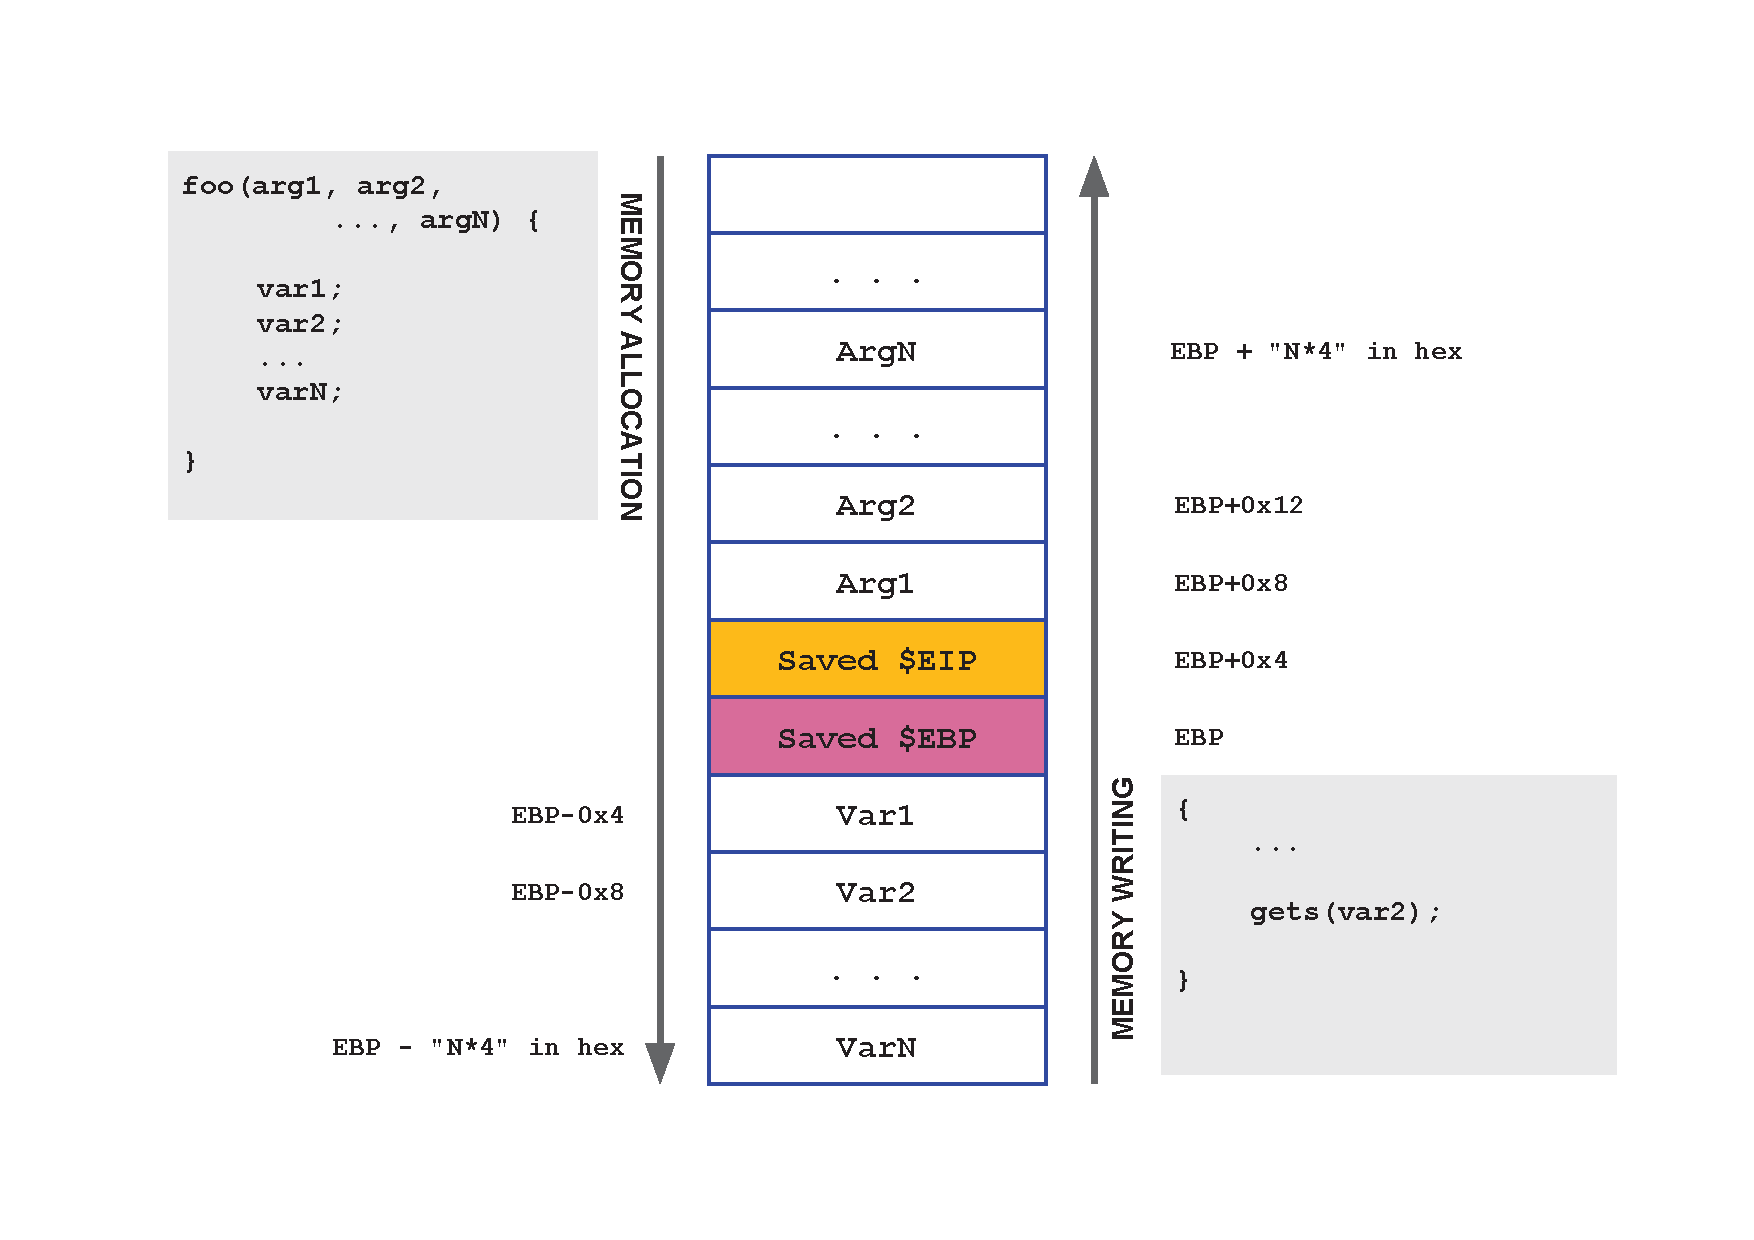
\includegraphics[width=\linewidth]{capitulo5/stack}
		\par\end{centering}
	\smallskip
	\caption[Pila de aplicación en Linux]{\label{fig:stack} Pila de aplicación en Linux. \cite{zanero_cs}}
\end{figure} 

\smallskip

Linux administra la pila en orden \textbf{descendente} (hacia direcciones de memoria menores). En cada llamada a función, se almacena el puntero de instrucción actual ---\acrshort{EIP}, \textit{\acrlong{EIP}}--- Si el \textit{buffer} de recepción está emplazado en la pila y se intenta escribir más allá de su longitud declarada, se sobrescribirá cualquier variable antes declarada. En el peor caso se modificará el puntero de instrucción guardado, causando una \textbf{violación de segmento} a la hora de retornar a la función anterior.

Más aún, este riesgo podría ser aprovechado por un \textbf{intruso} para modificar las instrucciones del programa, accediendo ilegalmente al sistema.

\smallskip

\begin{figure}[H]
	\noindent \begin{centering}
		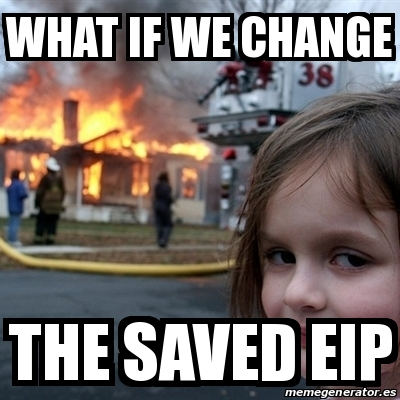
\includegraphics[width=\linewidth/2]{capitulo5/disaster_girl}
		\par\end{centering}
	\smallskip
	\caption{\label{fig:disaster_girl} ¿Y si cambiamos el puntero de instrucción?}
\end{figure} 

\smallskip

La \textbf{solución} adoptada es utilizar una cantidad razonable de memoria y limitar la cadena de entrada acotando tanto la \textbf{recepción} en la llamada al sistema \code{recv()} como la \textbf{comparación} de cadenas, usando \code{strncmp()} en lugar de \code{strcmp()}. Nuestro sistema utiliza \textit{buffers} de \textbf{4 \textit{KiB}}, memoria más que suficiente para recibir una lista de reproducción de tamaño considerable.

\subsubsection{Permisos de usuario}

Otra capa de seguridad se implanta utilizando permisos de usuario en el sistema de archivos de Linux, sobre el que descansa gran parte de la seguridad de este sistema operativo. Creamos el usuario \textbf{\code{organ}} y su grupo correspondiente, que serán \textbf{dueños} del proceso demonio y del \textit{socket}, con dos objetivos:

\begin{enumerate}
	\item Solo los usuarios autorizados (pertenecientes al grupo \code{organ}) podrán utilizar el \textit{socket}.
	
	\item En caso de intrusión, el servicio no podrá hacer en el sistema más cambios que los autorizados.
\end{enumerate}

Hay una excepción a tener en cuenta: el modo Ingeniería requiere\textbf{ apagar y reiniciar} el sistema. El programa \code{shutdown} requiere permisos de \textbf{superusuario}, pero es muy inseguro mantener el proceso con tales privilegios para tener esa capacidad.

Este problema se corrige modificando el archivo \code{/etc/sudoers}, que almacena la lista de usuarios que tienen permiso para utilizar la orden \code{sudo}. En él añadiremos al grupo \code{organ}, pero solo con capacidad de ejecutar \code{shutdown}, ningún otro programa.

\subsubsection{Conexiones simultáneas}

El núcleo de control del demonio es el planificador, que tiene una hebra independiente para reproducir piezas musicales. Los problemas de seguridad concurrente encontrados fueron descritos más arriba (sección \ref{subsec:impl_planificador}).

Sin embargo, surge un nuevo problema: sus funciones públicas pueden ser llamadas desde cualquier otro módulo, y cada uno de ellos funciona en una hebra distinta. Si dos funciones del planificador son ejecutadas \textbf{simultáneamente} se puede producir una inconsistencia o una \textbf{condición de carrera}.

Por ello, toda función pública está protegida por un \textbf{cerrojo} de exclusión mutua, a modo de monitor del módulo, que hace que cualquier subproceso que intente acceder deba esperar a que termine cualquier otra función que se esté ejecutando.

\subsection{Pre-instalación}

Para facilitar la compilación y la puesta en marcha del demonio, vamos a construir un \textit{script} que prepare el sistema para el funcionamiento del servicio, instalando los paquetes necesario y haciendo las configuraciones pertinentes.

El \textit{script} es muy sencillo y hace lo siguiente:

\begin{enumerate}
	\item Instala la biblioteca cliente de \textbf{MySQL} para C, incluyendo las cabeceras.
	\item Crea un usuario y grupo de sistema, llamados \code{organ}, que poseerán el proceso del demonio y el \textit{socket}.
	\item Agrega al usuario por defecto del \textit{Raspberry Pi} al grupo \code{organ}.
	\item Declara en el archivo \code{/etc/sudoers} permiso del grupo \code{organ} para ejecutar \code{shutdown}.
	\item Descarga la biblitoeca \textbf{WiringPi} del repositorio de su desarrollador, y la compila.
	\item Crea las carpetas \textbf{bin} y \textbf{obj}, para alojar los archivos compilados.
\end{enumerate}

\subsection{Compilación e instalación}

La compilación y la instalación del servicio está gestionada \textbf{\textit{Makefile}}, que trabaja sobre la siguiente estructura de directorios:

\begin{description}
	\item[bin] Archivos ejecutables finales.
	\item[include] Ficheros de cabecera de C.
	\item[obj] Código objeto, ensamblado pero no vinculado.
	\item[scripts] Código de pre-instalación y arranque del demonio.
	\item[src] Ficheros de código fuente en C.
\end{description}

El \textit{Makefile} contiene las siguientes reglas:

\begin{description}
	\item[all] Por defecto. Compila todos los ejecutables.
	\item[install] Instala los archivos compilados en el sistema operativo.
	\item[uninstall] Deshace la instalación.
	\item[preinstall] Ejecuta los pasos de pre-instalación.
	\item[clean] Elimina todos los archivos compilados.
	\item[objclean] Limpia los ficheros de código objeto.
\end{description}

Las carpetas utilizadas como destino de instalación son las siguientes:

\begin{description}
	\item[/usr/local/bin] Programas auxiliares.
	\item[/usr/local/sbin] Ejecutable del demonio (binarios de superusuario).
	\item[/etc/init.d] \textit{Script} de inicio del servicio.
\end{description}

\newpage

\section{Interfaz web}

Es ahora el momento de abordar la construcción del \textit{back-end} del sistema. Como ya sabemos, será un servidor \acrshort{HTTP}. Hemos tenido en cuenta las siguientes \textbf{alternativas} como lenguajes de programación para el servidor:

\begin{itemize}
	\item \textbf{C/C++ con \acrshort{CGI}}. Sería la solución más rápida en tiempo de ejecución, por ser lenguajes compilados. A cambio, la programación sería mucho más lenta, porque trabajamos a más bajo nivel.
	
	\item \textbf{\acrshort{PHP} 5}. Es quizás la opción más popular, es un lenguaje interpretado y diseñado para entornos \textit{web}.
	
	\item \textbf{Python 3 con la biblioteca Django}. También es un lenguaje interpretado, la biblioteca Django tiene una estructura más complicada, diseñada para sitios complejos.
\end{itemize}

Estudiadas las tres opciones, consideramos que la mejor es \textbf{\acrshort{PHP}}, por equilibrar rendimiento y comodidad de programación. En el capítulo posterior probaremos el tiempo de ejecución de las páginas, que es más que aceptable.

El servidor generará una página \textbf{\acrshort{HTML} 5}, la última versión del estándar. La estética se escribirá en \textbf{\acrshort{CSS} 3}. En el lado del cliente, siempre es necesario actuar sobre una página generada, donde utilizaremos \textbf{JavaScript} para acceder a ella a través de \acrshort{DOM} ---\textit{\acrlong{DOM}}---.

Además, debemos almacenar las cadenas constantes en archivos, dependiendo del idioma del usuario; para esto usaremos archivos \textbf{\acrshort{XML}}. Otra tecnología que nos resultará útil es \textbf{\acrshort{AJAX}} ---\textit{\acrlong{AJAX}}---, para que JavaScript haga consultas al servidor sin recargar la página completa.

En resumen usaremos las siguientes tecnologías:

\begin{enumerate}
	\item \acrshort{PHP} 5.4, como lenguaje de programación.
	\item \acrshort{HTML} 5, como lenguaje de marcado.
	\item \acrshort{CSS} 3, para las hojas de estilos.
	\item \acrshort{XML}, para almacenar información estática.
	\item JavaScript, \acrshort{AJAX} y \acrshort{DOM}, para interactuar dinámicamente con la página.
\end{enumerate}

\subsection{Estructura principal}

Vamos a organizar los archivos de una forma limpia y fácil de acceder. Para ello, en la carpeta raíz tendremos los archivos \acrshort{PHP} correspondientes a las vistas, y otro para el control. Cada \textbf{vista} se implementará en un archivo diferente, para facilitar la consulta. Ya que el \textbf{controlador} recibirá datos privados, se implementará en un solo archivo.

El resto de ficheros se clasificarán de las siguientes carpetas:

\begin{description}
	\item[ajax] Páginas \acrshort{PHP} de uso exclusivo para \acrshort{AJAX}.
	\item[images] Imágenes para la página.
	\item[lib] Bibliotecas \acrshort{PHP}, para el modelo y para la vista.
	\item[scripts] Código JavaScript a cargar por las páginas.
	\item[styles] Hojas de estilos en cascada, en \acrshort{CSS}.
	\item[translations] Ficheros de traducción, en \acrshort{XML}.
\end{description}

\subsubsection{Plantillas}

A medida que construimos la maqueta en \acrshort{HTML} y \acrshort{CSS}, fuimos conscientes de qué trozos de código se repetían, totalmente o con un ligero cambio, lo que nos ayudó a crear una \textbf{biblioteca de plantillas}, que podríamos denominar ''rutinas de vista''.

En ella hemos escrito las siguientes funciones:

\begin{description}[style=nextline]
	\item[\code{html\_open(id, refresh)}]
	Genera la cabecera \acrshort{HTML}. Establece el \code{id} del documento, y opcionalmente, una \acrshort{URL} de redirección (\code{refresh}).
	
	\item[\code{html\_close()}]
	De manera contraria, escribe el final del documento \acrshort{HTML}.
	
	\item[\code{html\_header(full)}]
	Modela la barra de cabecera. Si se indica \code{full} se hace completa, incluyendo los controles de energía (apagar y reiniciar). Si se pasa el valor \code{false}, entonces solo se muestra el cambio de idioma.
	
	\item[\code{html\_navigation (selected)}]
	Escribe la barra de navegación, marcando como seleccionado aquel elemento de la lista cuyo ID coincida con el valor de \code{selected}.
	
	\item[\code{html\_footer}]
	Muestra el pie de página de la vista.
	
	\item[\code{html\_error (type)}]
	Genera una página completa con un mensaje de error, y cuyo texto depende del parámetro \code{type}. A continuación termina el programa.
	
	\item[\code{html\_redirect (target)}]
	Crea una página sin contenido, dedicada a redireccionar a otra, cuya \acrshort{URL} se indica en \code{target}.
	
	\item[\code{html\_script (src)}]
	Escribe el texto \acrshort{HTML} necesario para incluir el archivo JavaScript especificado en \code{src}.
\end{description}

\subsubsection{Controlador}

Este archivo implementará todas las funciones de control del sistema, como iremos describiendo más adelante. Tan solo especificar que la ejecución de este módulo se lleva a cabo con una mezcla de parámetros \textit{GET} y \textit{POST}:

\begin{description}
	\item[GET] Solo se envía el nombre de la acción a ejecutar, como \code{control.php?action=login}.
	\item[POST] Transmite el resto de la información, cuyos parámetros dependen de la acción.
\end{description}

De esta forma se evita que el explorador o eventualmente un motor de búsqueda cacheen una instancia. Si la orden se ejecuta correctamente, se devuelve una página en blanco con \textbf{redirección} a la vista adecuada (se pierde la dirección y no se relanza la orden si actualizamos la página). En caso de \textbf{error}, se muestra pero se mantiene la dirección en el explorador para poder volver a intentarlo.

\subsubsection{Sesión}

Este módulo implementa el modelo de la sesión para permitir que todos los parámetros a almacenar sean accedidos por el resto de archivos a través de funciones, evitando errores lógicos. La interfaz está descrita en la sección \ref{subsec:session}, del capítulo de diseño.

La sesión de usuario es una \textbf{\textit{cookie}} gestionada por el intérprete de \acrshort{PHP}, que se incluye en la cabecera \acrshort{HTTP} al principio del programa, llamando a \code{session\_start()}. A partir de ahí, tenemos acceso a la variable global \code{\_SESSION}, un \textit{array} del que utilizaremos tres claves:

\begin{description}
	\item[auth] Tiene el valor 1 si el usuario se ha autentificado. Se escribe con \code{set\_auth()} y \code{unset\_auth()} y se consulta con \code{get\_auth()}.
	
	\item[last] Hace referencia a la consulta de la última vista ejecutada, por si el controlador debe volver a ella. Se escribe con \code{set\_page()} y se lee con \code{last\_page()}.
	
	\item[lang] Almacena el código de lenguaje seleccionado por el usuario o, en su defecto, el idioma preestablecido. Se escribe con \code{set\_language()} y se consulta con \code{get\_language()}.
\end{description}

\subsubsection{Hoja de estilos}

El modelo estándar de implementación de páginas \acrshort{HTML} separa contenido y forma en distintos archivos, así, todo el estilo de la interfaz se escribe en hojas de estilos en cascada.

Nuestra interfaz será \textbf{homogénea}, de manera que todos los estilos se definirán en un solo archivo \acrshort{CSS}. El objetivo es obtener un resultado lo más cercano posible al diseño, donde tenemos un ejemplo en la figura \ref{fig:maqueta}.

Sin adentrarnos en el código, existen tres zonas bien distinguidas en el fichero:

\begin{enumerate}
	\item Reglas \textbf{generales}, como el margen, la tipografía o el color de la fuente.
	\item Opciones para los \textbf{elementos}, dependiendo de su etiqueta \acrshort{HTML}.
	\item Reglas \textbf{específicas}, sobre todo a determinadas páginas. Esta es la razón por la que cada vista tiene un ID diferente.
\end{enumerate}

Como podemos ver en las siguientes figuras, hemos conseguido una estética en \acrshort{CSS} prácticamente similar a la diseñada con Photoshop.

\subsection{Traductor}

El traductor es el módulo en el que delegamos todo el texto que aparecerá en las \textbf{vistas} y será dependiente del idioma que escoja el usuario. Como especificamos en la sección \ref{subsec:idiomas} del capítulo de diseño, cada archivo de traducción implementará un elemento \code{<translation>} como raíz, dedicado a un solo lenguaje.

Un ejemplo para un ''Hola Mundo'' en dos idiomas sería el siguiente:

\begin{Verbatim}[commandchars=\\\{\}]
	\color{blue}<translation \color{red}code\color{black}=\color{violet}"es" \color{red}language\color{black}=\color{violet}"Español"\color{blue}>
	    \color{blue}<string \color{red}name\color{black}=\color{violet}"hello"\color{blue}>\color{black}¡Hola Mundo!\color{blue}</string>
	\color{blue}</translation>

	\color{blue}<translation \color{red}code\color{black}=\color{violet}"it" \color{red}language\color{black}=\color{violet}"Italiano"\color{blue}>
		\color{blue}<string \color{red}name\color{black}=\color{violet}"hello"\color{blue}>\color{black}Ciao Mondo!\color{blue}</string>
	\color{blue}</translation>
\end{Verbatim}

El programa en \acrshort{PHP} busca todos los archivos existentes en la carpeta de traducciones con \code{glob()} y los interpreta con ayuda de la función \code{simplexml\_load\_file()}. A continuación los guarda en una lista global, denominada \code{translators}, a acceder por todas las funciones que la requieran.

El hecho de leer todos los archivos de lenguaje se explica en el \textbf{menú desplegable} que se mostrará en la barra de cabecera, y presenta todos los idiomas disponibles, con el siguiente aspecto:

\smallskip

\begin{figure}[H]
	\noindent \begin{centering}
		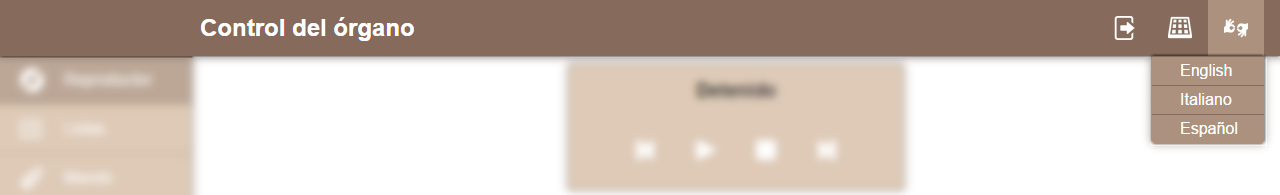
\includegraphics[width=\linewidth*3/4]{capitulo5/cap_repr_idiomas}
		\par\end{centering}
	\smallskip
	\caption{\label{fig:cap_repr_idiomas} Vista del menú desplegable de idiomas.}
\end{figure} 

\smallskip

Cada opción está vinculada al \textbf{controlador}, que lanza la orden \code{language} con el código de idioma como parámetro.

\subsection{Control de energía}

Una de las funciones de la interfaz sería controlar el reinicio y el apagado del \textit{Raspberry Pi}. Esta acción solo se puede llevar a cabo con la orden correspondiente de Linux, y con permiso de superusuario.

La implementación es tan sencilla como mostrar en la cabecera un \textbf{menú desplegable} con ambas opciones:

\smallskip

\begin{figure}[H]
	\noindent \begin{centering}
		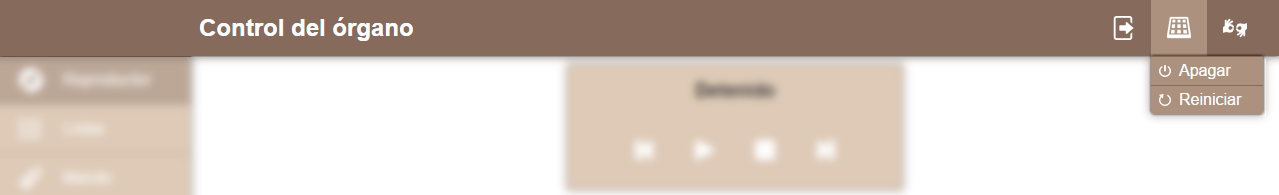
\includegraphics[width=\linewidth*3/4]{capitulo5/cap_repr_apagar}
		\par\end{centering}
	\smallskip
	\caption{\label{fig:cap_repr_apagar} Vista del menú desplegable de control de energía.}
\end{figure} 

\smallskip

Cada uno de estos elementos llama a controlador con una acción diferente:

\begin{description}
	\item[shutdown] Hace ejecutar la función \code{shutdown()}, que solo llama a \code{sudo shutdown now}.

	\item[reboot] Ejecuta la función \code{reboot()}, que llama a \code{sudo shutdown -r now}.
\end{description}

Ambas llamadas devuelven un \textbf{código de retorno} (0 en caso de éxito o 1 en caso de error). El controlador filtra dicho código para \textbf{redirigir a la portada}, o bien mostrar un mensaje de error.

Recordar que el usuario del servidor Apache (www-data) no posee por defecto privilegios para realizar cambios que afecten al equipo. Por ello modificaremos el sistema para concederle tales permisos, como explicaremos más adelante, en la sección \ref{subsec:web_seguridad}.

\subsection{Portada}
\label{subsec:impl_portada}

La portada constituye la primera página que se muestra al acceder al sistema. La \textbf{vista} incluye un fondo de pantalla dinámico, que cambia a intervalos de tiempo regulares.

Para esto hemos implementado una función en JavaScript llamada \code{toggle()}, que guarda una lista de imágenes y altera el estilo del fondo de la página.

Otro elemento importante es un \textbf{formulario} que permite introducir la contraseña de usuario y nos lleva al \textbf{controlador}, con la acción \code{login}.

\subsubsection{Autentificación}

El \textbf{controlador} recibe la contraseña por el método \textit{POST}, para ocultarla de la vista de la dirección y evitar que sea cacheada. Todo lo que hará será llamar a una \textbf{aplicación auxiliar} de la que hablaremos más tarde, en la sección \ref{subsec:aux_login}. A esta aplicación le pasamos el nombre de usuario (predefinido por nosotros) y la contraseña introducida como parámetros de llamada, y nos devuelve 0 (correcto) o 1 (error).

Si se aprueba el acceso, llamamos a \code{set\_auth()} para registrarlo en la sesión y redirigimos al \textbf{reproductor}. En caso contrario, volvemos a la pantalla con parámetro \code{error=1}, de forma que se mostrará un pequeño mensaje de error:

\smallskip

\begin{figure}[H]
	\noindent \begin{centering}
		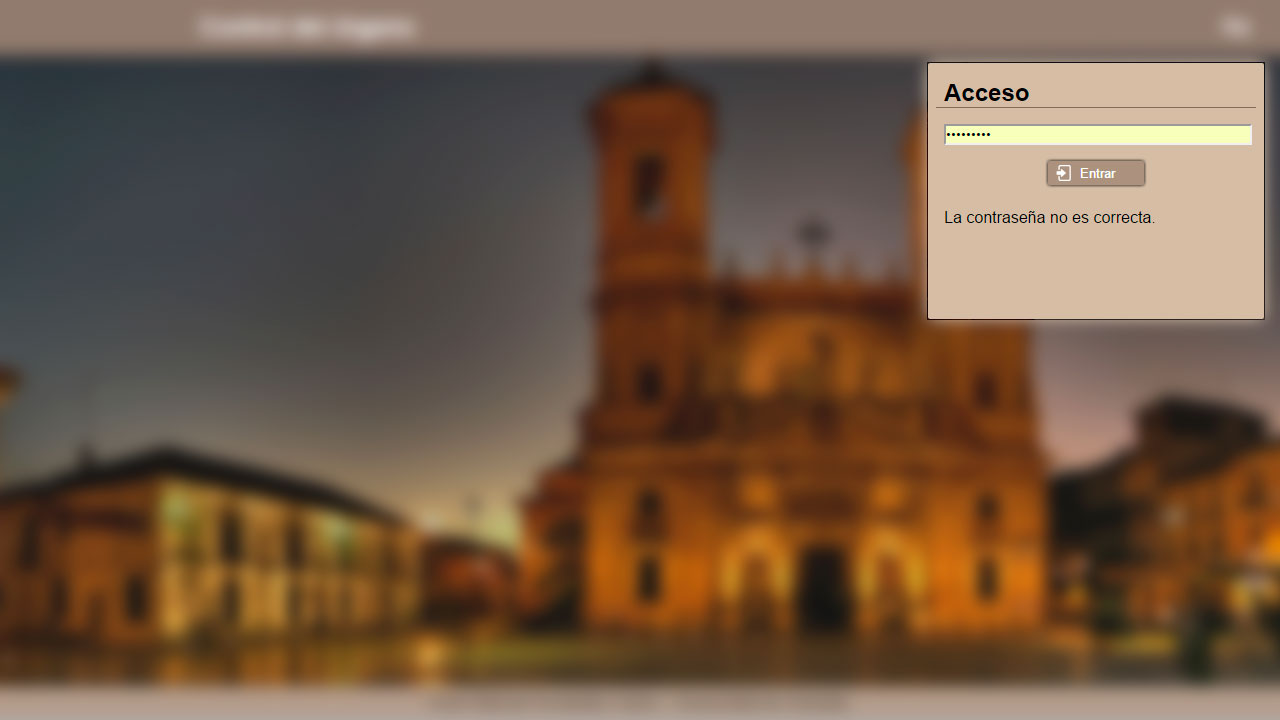
\includegraphics[width=\linewidth*3/4]{capitulo5/cap_login_error}
		\par\end{centering}
	\smallskip
	\caption{\label{fig:cap_login_error} Formulario de entrada con mensaje de error.}
\end{figure} 

\smallskip

Por razones de seguridad, la utilidad de autentificación \textbf{retrasa} la ejecución 2 segundos en caso de recibir una contraseña incorrecta, atenuando la efectividad de un \textbf{ataque por fuerza bruta}.

\subsection{Navegación}

Para movernos cómodamente entre las páginas de la interfaz, hemos diseñado una barra lateral de navegación. Consiste en una lista de vínculos, adornados con iconos mediante estilos. 

La función de la plantilla que la crea, \code{html\_navigation()}, utiliza el ID de la página para indicar la clase \code{selected} al vínculo correspondiente. La hoja de estilos se encarga de que dicho elemento se dibuje de otro color para remarcar la página actual.

\smallskip

\begin{figure}[H]
	\noindent \begin{centering}
		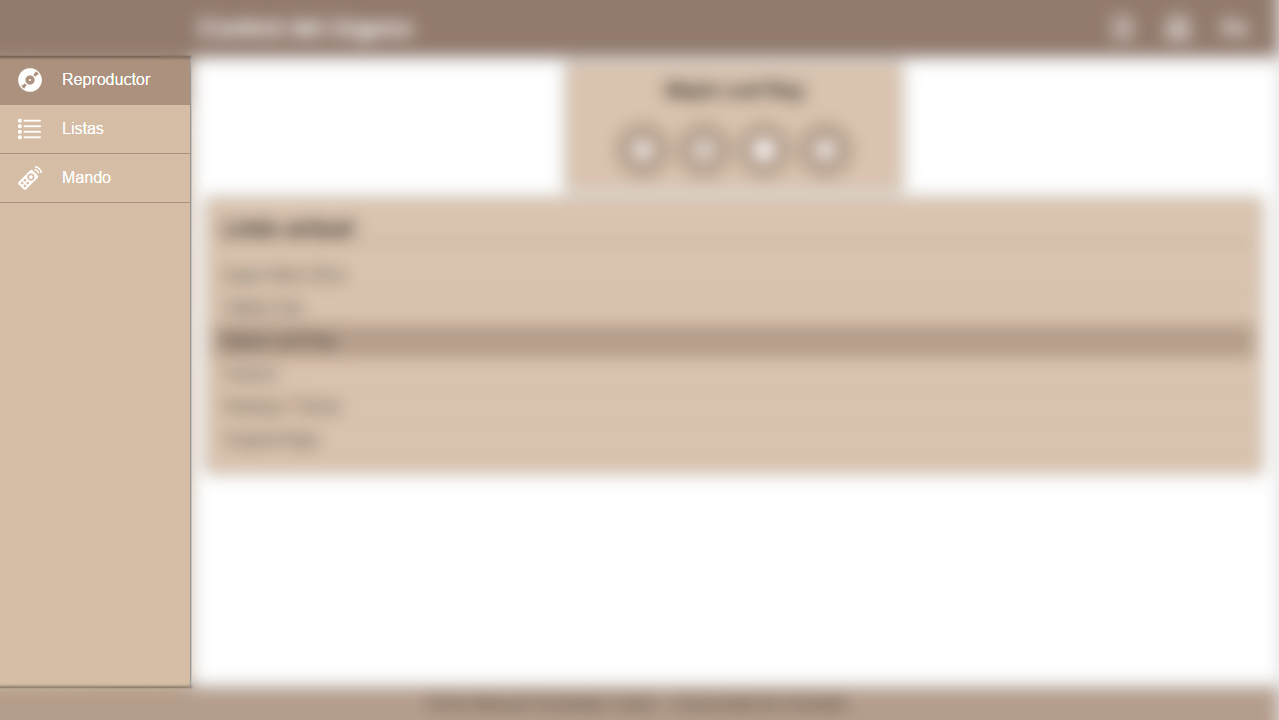
\includegraphics[width=\linewidth*3/4]{capitulo5/cap_navigation}
		\par\end{centering}
	\smallskip
	\caption{\label{fig:cap_navigation} Barra lateral de navegación.}
\end{figure} 

\smallskip

\subsection{Conexión a la base de datos}

De manera análoga a como hicimos en el demonio para comunicarnos con la base de datos independientemente del motor utilizado, en la interfaz dedicaremos un módulo a conectarnos a la base de datos MySQL.

La estructura de datos que más utilizaremos serán \textbf{mapas asociativos} (\textit{arrays} con claves), ya que son la estructura subyacente en los objetos de \acrshort{PHP} y, por consiguiente, más eficientes.

Nuestro módulo establecerá una conexión con la base de datos, creando un objeto \code{mysqli}, la nueva versión del cliente MySQL para \acrshort{PHP}. Las credenciales y el nombre de esquema quedan predefinidos mediante constantes. En caso de \textbf{error}, se mostrará un mensaje con \code{html\_error()}, y no podremos continuar hasta que solucionemos el problema.

Todas las funciones definidas están descritas en la sección \ref{subsec:web_database} de diseño. El \textbf{procedimiento habitual} para ejecutar una sentencia es el siguiente:

\begin{enumerate}
	\item Creamos una sentencia preparada con \code{prepare()}, a partir del código SQL correspondiente, marcando con una interrogación ('?') los valores que irán parametrizados.
	\item Utilizamos el método \code{bind\_param()} para enlazar cada parámetro con su argumento correspondiente, que recibiremos en la llamada a la función.
	\item Ejecutamos la sentencia con el método \code{execute()}.
	\item Recibimos la información requerida con \code{get\_result()}.
	\item Clasificamos los datos según sea necesario, y los devolvemos.
\end{enumerate}

\subsection{Conexión al demonio}

Si el demonio implantaba un servidor de \textit{socket}, nosotros vamos a escribir un \textbf{cliente} que se conecte a él. El código de inicio utiliza las funciones \code{socket\_create()} y \code{socket\_connect()} para establecer una conexión con el \textit{socket} del demonio, sito en \code{/run/organ.sock}.

El resto de funciones simplemente adaptan la llamada correspondiente a una orden que siga el \textbf{protocolo} descrito en la sección \ref{sec:protocolo}. Las interfaz de las funciones se desglosó en la sección \ref{subsec:web_demonio}, donde diseñamos este módulo.

\code{driver\_play()} recibe una lista de reproducción (obtenida de la base de datos) y el índice de la primera pieza. Entonces \textbf{genera la cadena} de nombres de archivo, empezando por la partitura indicada, y la envía al demonio.

\code{driver\_pause()}, \code{driver\_resume()} y \code{driver\_stop()} simplemente \textbf{transmiten la orden} procedente y reciben el mensaje de retorno, que indica si se ha realizado correctamente la operación. Los casos típicos de fallo son:

\begin{enumerate}
	\item Tener un estado incompatible con la llamada (e.g. pausar si estaba detenido).
	\item Estar en modo Ingeniería.
\end{enumerate}

Por último, \code{driver\_status()} lanza una consulta y devuelve los datos recibidos tal cual en un array con el siguiente contenido:

\begin{enumerate}
	\item Palabra de estado, en mayúscula ---como dicta el protocolo---.
	\item Ruta absoluta de la pieza que se está reproduciendo (si procede).
\end{enumerate}

\subsection{Reproductor}

Ésta es la página principal del administrador, desde la que podremos controlar la reproducción del órgano. Tendrá la funcionalidad básica de cualquier reproductor.

\subsubsection{Vista}

La página se genera en función de una consulta hacia el \textbf{demonio} para conocer su estado, mediante \code{driver\_status()}. En caso de estar reproduciendo o en pausa, también recibimos la ruta absoluta del archivo MIDI en curso. Probablemente sea una pieza almacenada en la base de datos y, por consiguiente, perteneciente a una lista. O bien sea un archivo puntualmente ejecutado por consola.

\smallskip

\begin{figure}[H]
	\noindent \begin{centering}
		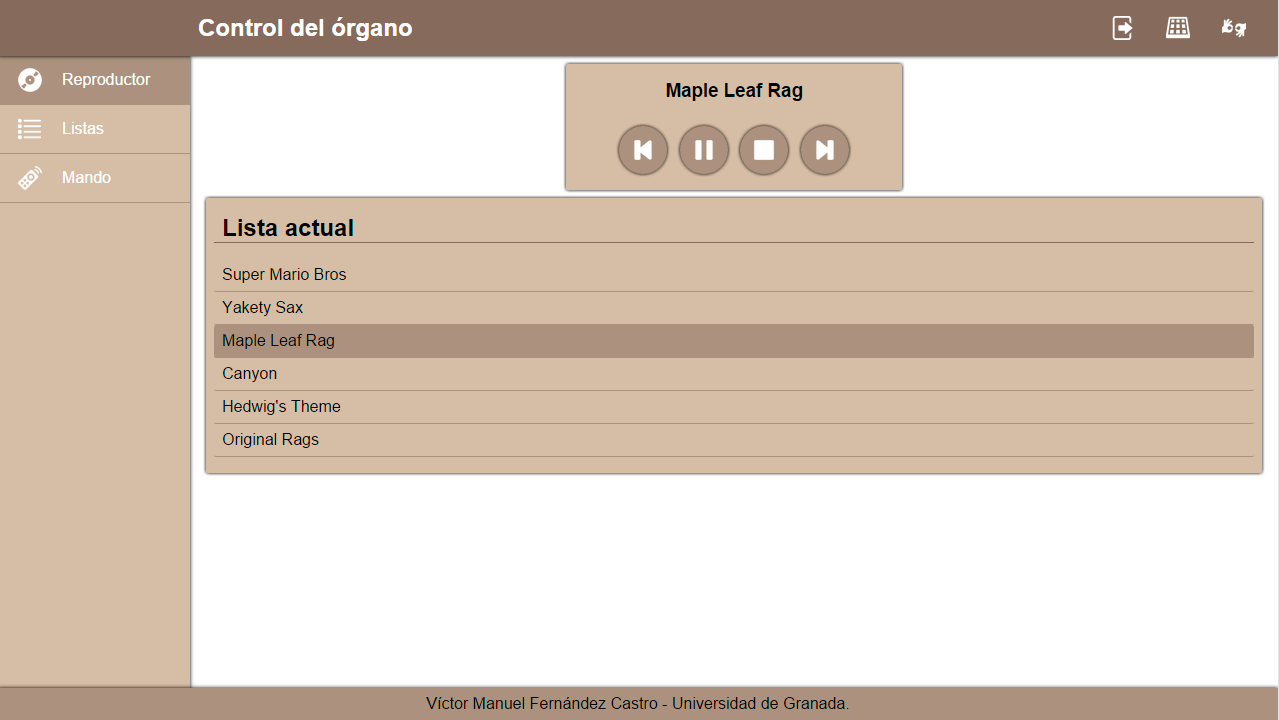
\includegraphics[width=\linewidth*3/4]{capitulo5/cap_reproductor}
		\par\end{centering}
	\smallskip
	\caption{\label{fig:cap_reproductor} Vista del reproductor.}
\end{figure} 

\smallskip

Si el reproductor recibe un nombre de archivo, lo busca en la base de datos e infiere inferir la lista que se está reproduciendo. Pueden ocurrir dos cosas:

\begin{enumerate}
	\item Si el archivo está registrado, muestra el título y la lista de reproducción correpondiente.
	\item Si no es encuentra el fichero, aparece el nombre de archivo y no se muestra ninguna lista.
\end{enumerate}

El resto de controles aparecen a razón del estado. Para cambiar la partitura a reproducir, podemos desplazar con los botones adelante/atrás, o bien \textbf{seleccionar} un elemento de la lista.

\subsubsection{Controlador}

El grueso del controlador de este módulo está compuesto por llamadas a funciones escritas en JavaScript que se comunican dinámicamente con el servidor utilizando \textbf{\acrshort{AJAX}}, para obtener una respuesta eficiente y evitar recargar la página. Cada botón está asignado a una función diferente:

\begin{description}
	\item[\code{resume()}] Reanudar la reproducción.
	\item[\code{pause()}] Pasar programa.
	\item[\code{stop()}] Detener completamente.
	\item[\code{previous()}] Siguiente pista, circularmente.
	\item[\code{next()}] Pista anterior, circularmente.
\end{description}

\code{pause()}, \code{resume()} y \code{stop()} hacen una petición de tipo \acrshort{AJAX} a pequeñas aplicaciones \acrshort{PHP} específicas a tal efecto, que simplemente transmiten la orden al demonio mediante el \textit{socket}. Después, modifican los controles según corresponda ---ocultar un botón, mostrar otro, etc.---

\code{previous()} y \code{next()}, para los botones adelante/atrás, realizan \textbf{peticiones completas} para reproducir una lista, empezando por una pista distinta. La reproducción se hace en ciclo, por tanto, la pieza que sucede a la última es la primera.

Este mismo mecanismo se utiliza cuando se pulsa sobre un elemento de la lista, que llama a la función de JavaScript \code{play()}. Todas ellas hacen al servidor una petición del tipo: 

\begin{center}
	\code{control.php ? action=play \& idplaylist=\$X \& idscore=\$Y}
\end{center}

La parte del control en \acrshort{PHP} recibe la orden, consulta en la base de datos la lista de archivos y la envía al demonio a través del \textit{socket}.

\subsection{Gestión de listas y piezas}
\label{subsec:impl_gestor}

Esta parte de la aplicación nos permite administrar las piezas almacenadas en el sistema, crear y modificar listas de reproducción, y gestionar las partituras que contienen.

\subsubsection{Vista}

El módulo consta de \textbf{dos vistas}: una para ver las \textbf{listas} existente y crear nuevas, y otra para gestionar las \textbf{piezas} contenidas en cada lista, a la que accedemos desde la primera página.

El gestor de listas consiste esencialmente en una \textbf{tabla} que muestra las listas que hemos creado, nos da a conocer el nombre y el número de piezas contenidas. Además proporciona un botón para \textbf{reproducir} directamente la lista. La página muestra también un botón para \textbf{insertar} una lista nueva.

\smallskip

\begin{figure}[H]
	\noindent \begin{centering}
		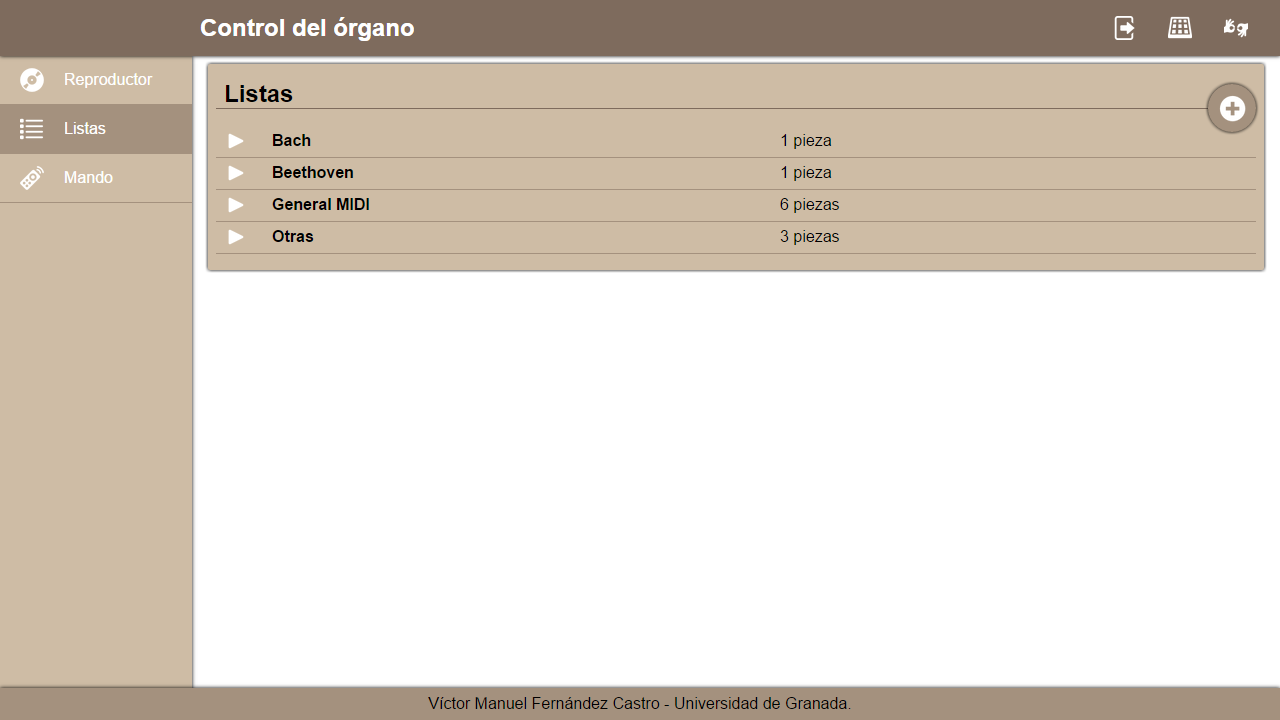
\includegraphics[width=\linewidth*3/4]{capitulo5/cap_listas}
		\par\end{centering}
	\smallskip
	\caption{\label{fig:cap_listas} Vista del gestor de listas.}
\end{figure} 

\smallskip

Para generar esta página, la aplicación hace una consulta a la \textbf{base de datos} llamando a \code{db\_get\_playlists()}, que devuelve un \textit{array} con todas las listas almacenadas. Hacer clic en cualquier lista nos lleva a la vista siguiente, para gestionarla.

Para \textbf{crear una lista}, el botón correspondiente llama a una función JavaScript, \code{add()}, que hace aparecer una \textbf{ventana modal} con un pequeño formulario para que introduzcamos el nombre de la nueva lista.

Por \textbf{seguridad}, el campo es obligatorio y está limitado a 255 caracteres, la misma longitud que la columna de la base de datos que almacenará esta información. Aún así, el \textbf{controlador} realizará una segunda comprobación cuando reciba los datos.

\smallskip

\begin{figure}[H]
	\noindent \begin{centering}
		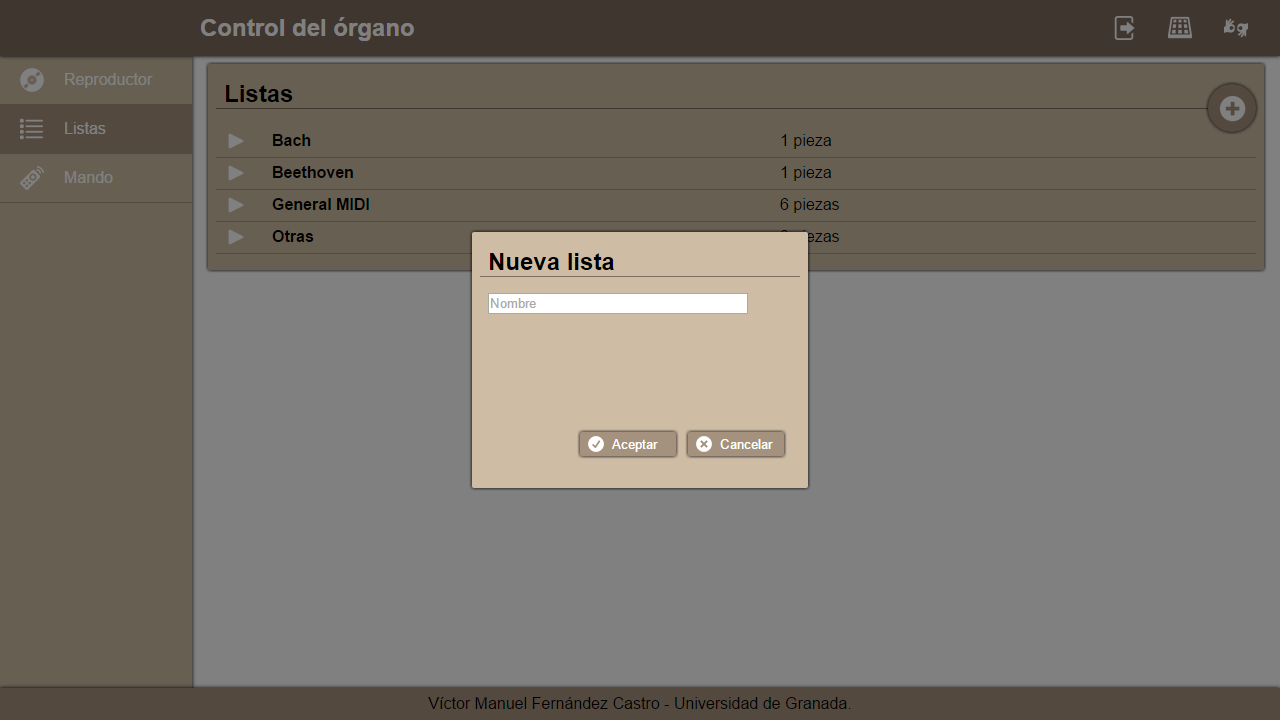
\includegraphics[width=\linewidth*3/4]{capitulo5/cap_ins_lista}
		\par\end{centering}
	\smallskip
	\caption{\label{fig:cap_ins_lista} Diálogo para crear una lista.}
\end{figure} 

\smallskip

El \textbf{administrador de piezas} es una vista similar al gestor de listas, pero en cambio muestra el contenido de cada lista. Se accede de forma normal haciendo clic en una lista de reproducción, que llama a esta vista con esta sintaxis:

\begin{center}
	\code{playlist.php ? idplaylist=\$X}
\end{center}

Esta página busca la lista indicada por ID en la base de datos y extrae su contenido mediante la función \code{db\_get\_playlist()}. A partir de esta información genera una tabla en la que a cada partitura le corresponde una fila, y nos da a conocer el título y la duración, también aparece un vínculo para descargar la pieza en formato \acrshort{MIDI}, un botón para cambiar el título y otro para eliminarla. 

La cabecera de la sección provee controles que permiten renombrar y borrar la lista, así como añadir una nueva pieza. Esta zona soporta ''\textbf{arrastrar y soltar}'' para añadir piezas fácilmente. La vista tiene el siguiente aspecto:

\smallskip

\begin{figure}[H]
	\noindent \begin{centering}
		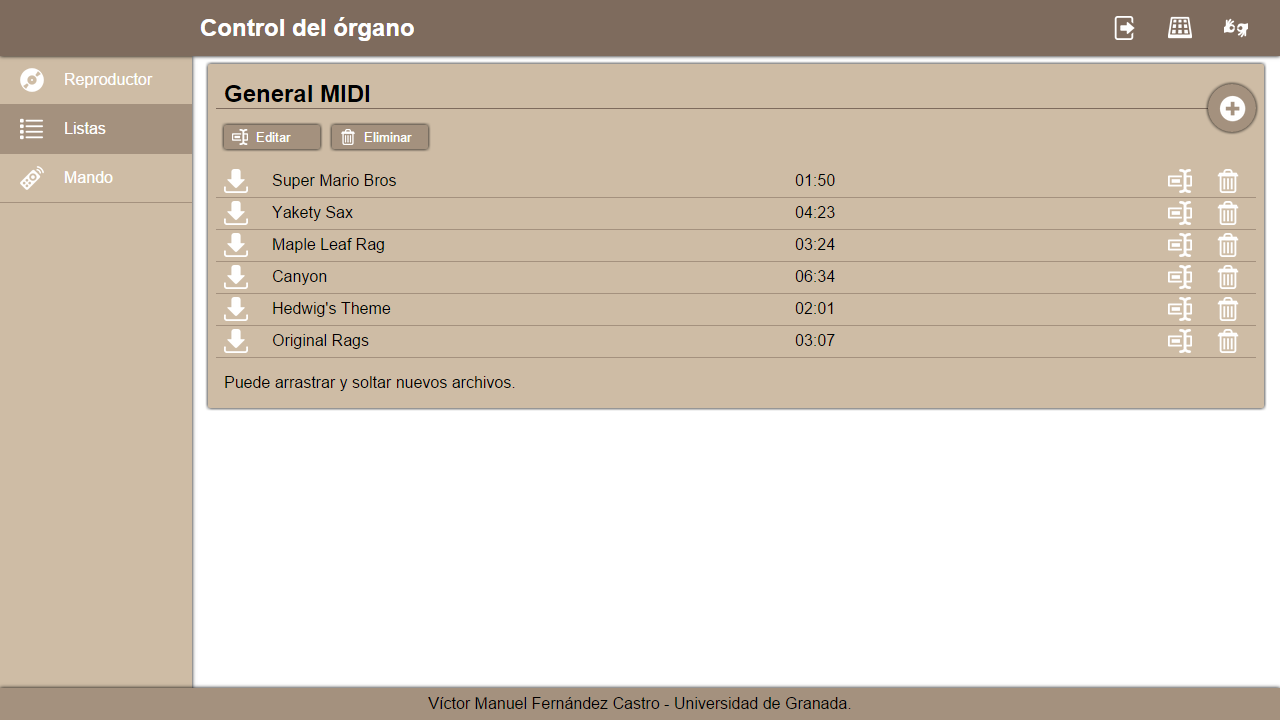
\includegraphics[width=\linewidth*3/4]{capitulo5/cap_piezas}
		\par\end{centering}
	\smallskip
	\caption{\label{fig:cap_piezas} Vista del administrador de piezas.}
\end{figure} 

\smallskip

Para \textbf{añadir una partitura} tenemos un botón de tipo \code{<input type=''file''>}, que tiene un comportamiento aislado por el navegador por razones de seguridad, y ni siquiera se puede cambiar su estilo. Por ello, este control está oculto y en su lugar aparece un botón  estándar, programado para transmitir la función \code{click()} cuando el usuario pulse sobre él. Al hacerlo, aparece un pequeño explorador para seleccionar un archivo, filtrado por formato \acrshort{MIDI}.

El vínculo para \textbf{descargar} enlaza al archivo correspondiente en el servidor, pero éste guarda el archivo con un nombre numérico para evitar colisiones. Por esta razón, se indica en el vínculo el \textbf{nombre de la pieza} para guardar el archivo descargado, si el navegador lo soporta.

Por último, existen varias \textbf{ventanas modales}, cada una correspondiente a un diálogo que se hará aparecer cuando el usuario haga clic en el botón correspondiente, mediante sencillas funciones JavaScript. En el caso de renombrar, el cuadro de texto adquiere el título actual de la pieza o de la lista, y adquiere el foco del teclado para agilizar la operación.

\smallskip

\begin{figure}[H]
	\noindent \begin{centering}
		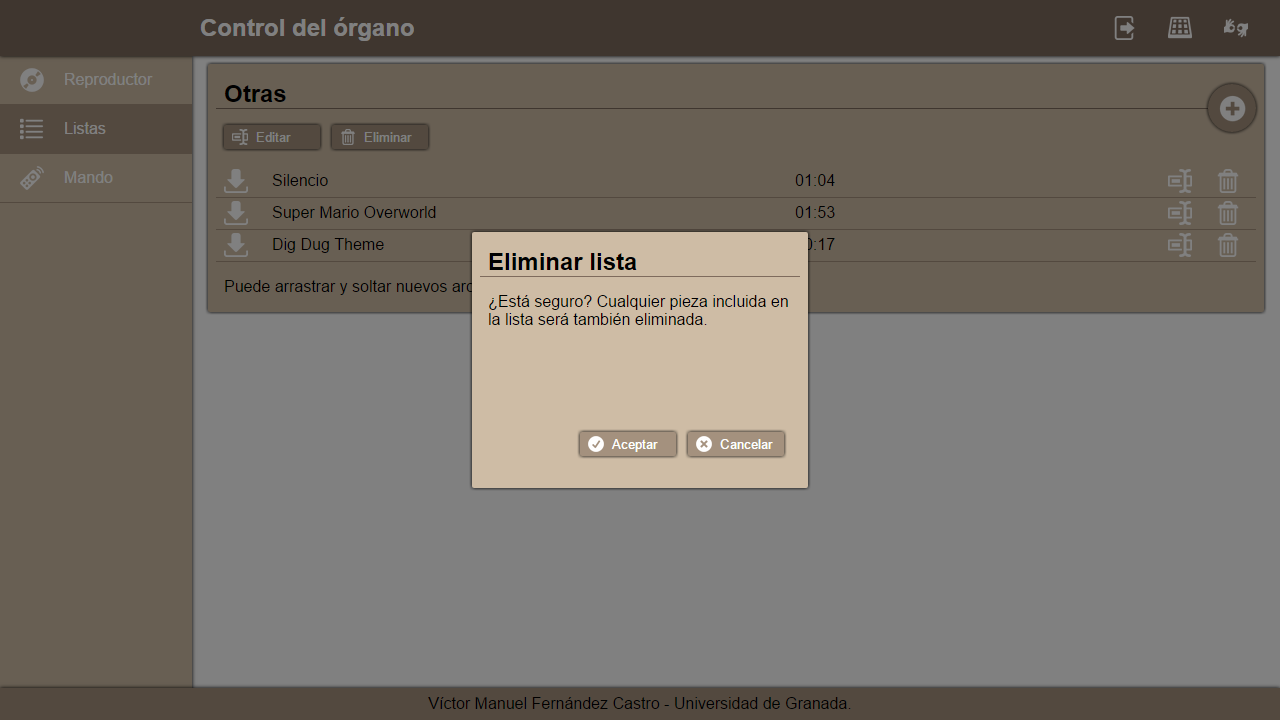
\includegraphics[width=\linewidth*3/4]{capitulo5/cap_elim_lista}
		\par\end{centering}
	\smallskip
	\caption{\label{fig:cap_elim_lista} Diálogo para eliminar una lista.}
\end{figure} 

\smallskip

\subsubsection{Controlador}

La mayor parte del controlador para este módulo consiste en pequeñas funciones de acceso a la base de datos. Su sintaxis está descrita en en las secciones \ref{subsec:listas} y \ref{subsec:piezas}:

\code{new\_playlist()}, \code{rename\_playlist()} y \code{rename\_score()} alteran la base de datos llamando a la función del modelo del mismo nombre. En todos los casos, se verifica que el título exista, si es mayor que el campo de la base de datos que lo almacena, será truncado.

\code{delete\_score()} borra una pieza de la base de datos y del almacenamiento. La función \code{delete\_playlist()} elimina una lista de la base de datos, pero antes debe obtener los nombres de archivos contenidos y eliminarlos. Ya que las listas están enlazadas a las piezas por \textbf{llave externa}, las tuplas correspondientes a las piezas contenidas en la lista se eliminarán automáticamente.

\code{new\_score()} inserta una pieza en una lista. Recibe el parámetro \code{idplaylist} y el archivo \acrshort{MIDI}. En primer lugar comprueba el formato del archivo y su tamaño ---se descartan archivos mayores de 1 \textit{MiB}--- y utiliza la aplicación \textit{Midinfo} (descrita en la sección \ref{subsec:midinfo}) para conocer su duración y verificar su formato. Para \textbf{evitar colisiones} de nombres, el archivo se guardará con un nombre igual a su identificador en la base de datos. La inserción se hace en dos pasos:

\begin{enumerate}
	\item Se inserta la tupla mediante \code{db\_insert\_score()}, que crea el elemento asignando como título el nombre original de archivo, pero establece otro nombre de almacenamiento único.
	
	\item Se mueve el archivo recibido a la carpeta específica para contener partituras, con el nombre de archivo que indica la base de datos.
\end{enumerate}

Como hemos explicado en la vista, hay \textbf{dos métodos} para subir archivos, aunque ambos llaman a la misma función del controlador:

\begin{enumerate}
	\item Seleccionando un archivo \acrshort{MIDI} en el explorador que aparece al pulsar el\textbf{ botón para añadir} una pieza. El archivo se envía en el formulario de manera normal. Solo se permite seleccionar un fichero y, de fallar, recibiremos un mensaje de error indicando los motivos.
	
	\item \textbf{Arrastrando} uno o varios archivos a la sección central de la vista. Esto activa la función \code{ondrop()} de JavaScript, que no puede acceder al elemento \code{<input>} del formulario mediante \acrshort{DOM} y añadir el archivo recibido, por motivos de seguridad. En cambio, utiliza \acrshort{AJAX} para hacer dinámicamente un envío por cada archivo. Ya que \acrshort{AJAX} es, por definición, \textbf{asíncrono}, enviaría todos los archivos simultáneamente. Para evitarlo, establecemos un \textit{callback} al recibir la respuesta, que haga transmitir el archivo siguiente. La implementación es similar a una \textbf{función recursiva}. Si un archivo falla, es descartado silenciosamente.
\end{enumerate}

\smallskip

\begin{figure}[H]
	\noindent \begin{centering}
		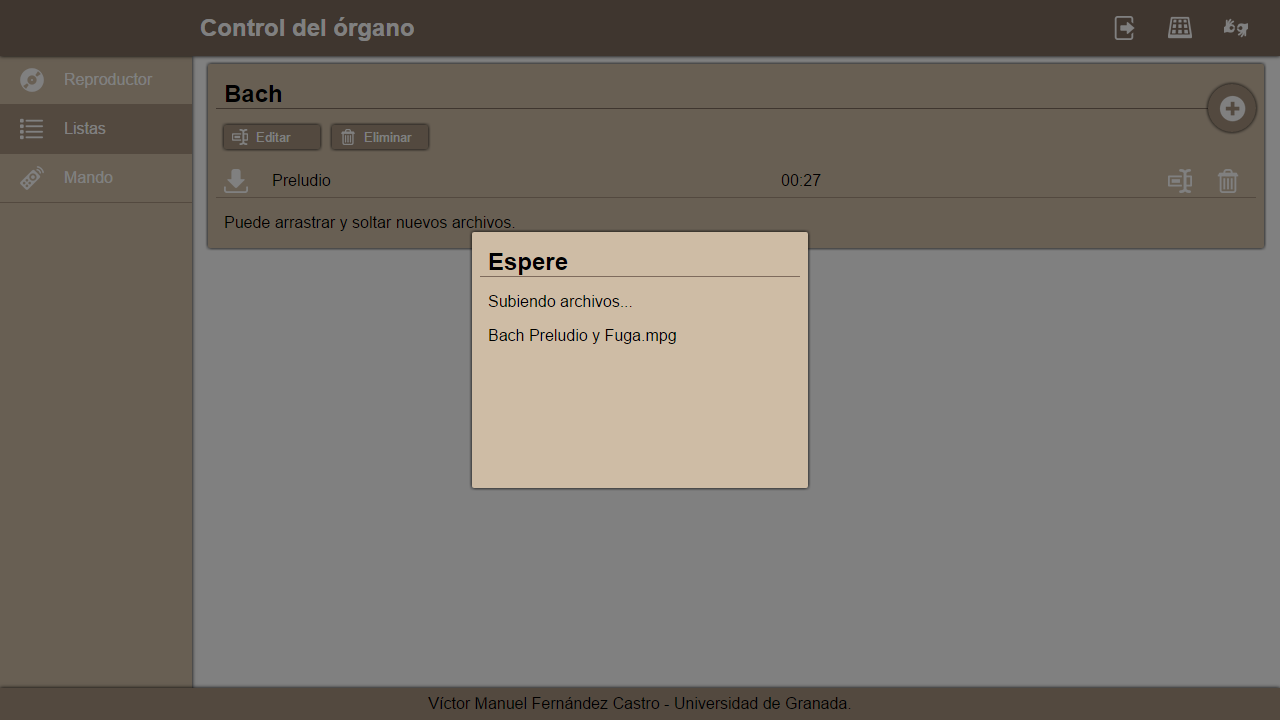
\includegraphics[width=\linewidth*3/4]{capitulo5/cap_ins_pieza}
		\par\end{centering}
	\smallskip
	\caption{\label{fig:cap_ins_pieza} Progreso de inserción de piezas.}
\end{figure} 

\smallskip

Este segundo método permite enviar muchos archivos y puede tardar algún tiempo, aunque la interfaz siga respondiendo. Mientras se están subiendo archivos aparece una ventana emergente que muestra qué fichero está en curso.

\subsection{Asignación del mando}

Una vez creadas las listas, tendremos la posibilidad de asignarlas a un botón del mando a distancia. La \textbf{base de datos} almacena esta información y permite que sea consultada directamente por el demonio, que será el que reciba las pulsaciones del mando.

\subsubsection{Vista}

Esta página muestra una \textbf{tabla} con todos los botones contemplados en el mando, y la lista que tiene asignada cada uno. Este dato viene dado en un \textbf{menú desplegable} que da a escoger entre todas las listas recogidas en la base de datos, o dejar el botón \textbf{sin asignar}.

\smallskip

\begin{figure}[H]
	\noindent \begin{centering}
		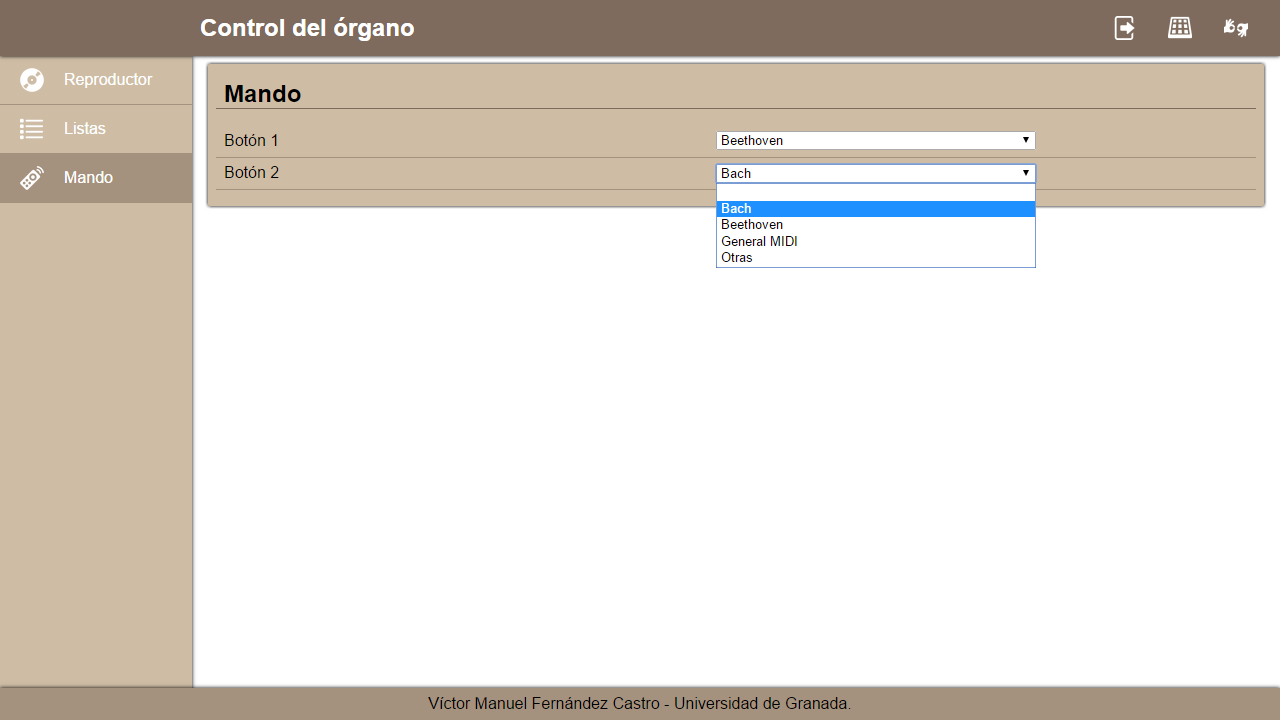
\includegraphics[width=\linewidth*3/4]{capitulo5/cap_mando}
		\par\end{centering}
	\smallskip
	\caption{\label{fig:cap_mando} Vista del gestor del mando.}
\end{figure} 

\smallskip

\subsubsection{Controlador}

Para establecer un vínculo entre un botón y una lista, el controlador ejecuta la función \code{set\_shortcut()}. Como se describió en la sección \ref{subsec:mando} de diseño, recibe el identificador de botón y de lista.

El controlador hace patente la asignación en la base de datos llamando a la función del modelo, \code{db\_set\_shortcut()}, dejando automáticamente la información compartible hacia el servicio de reproducción.

\subsection{Seguridad}
\label{subsec:web_seguridad}

Si en el \textit{back-end} los detalles de seguridad que nos preocupaban son esencialmente los relacionados con incompatibilidades del formato \acrshort{MIDI}, permisos de usuario y gestión de la concurrencia, ahora debemos atender escrupulosamente la \textbf{entrada de datos} provenientes del usuario que, de forma intencional o no, podría causar un error en el sistema.

En el \textit{front-end} implantaremos dos capas de seguridad:

\begin{enumerate}
	\item Una primera capa en la \textbf{vista}, para informar inmediatamente de un error en un formulario.
	\item Otra capa en el \textbf{controlador}, para evitar errores más complejos o un conjunto de datos forzado.
\end{enumerate}

\subsubsection{Cadenas de entrada}

Los formularios de la aplicación proveen \textbf{campos de texto} para introducir ciertos datos, como el nombre de una partitura. La información llega a la base de datos, cuyos campos están limitados, generalmente a 255 \textit{bytes}, y son obligatorios.

Para conseguir la mayor efectividad, los campos \code{<input>} tienen marcadas estas condiciones, para alertar al usuario. Sin embargo, pueden ser forzados fácilmente con las \textbf{funciones de depuración} del explorador. Dichas condiciones son comprobadas de nuevo en el \textbf{controlador}; en caso de no cumplirse, se muestra un error.

\subsubsection{Formato de archivo MIDI}

El único tipo de archivo aceptado para guardar partituras en el sistema es el formato \acrshort{MIDI}. De manera similar al caso anterior, el explorador desplegado a la hora de añadir partituras filtra los archivos por extensión, pero esta medida es fácilmente sorteable.

Como especificamos más arriba (sección \ref{subsec:impl_gestor}), el controlador del gestor de piezas llama al \textbf{analizador} de archivos \acrshort{MIDI} antes de insertar el fichero. Si la aplicación no reconoce el archivo \textbf{completamente}, devuelve un error y se descarta.

\subsubsection{Inyección de código SQL}

Un error de programación muy común al comunicar el controlador con el modelo es \textbf{concatenar} una orden con la entrada del usuario. Por ejemplo, para buscar un usuario en la base de datos para autentificar:

\begin{center}
	\code{SELECT id FROM user WHERE nick = '\$X' AND password = '\$Y'}
\end{center}

Si el usuario escribe en el campo de contraseña el siguiente texto:

\begin{center}
	\framebox[\textwidth/4][c]{\code{' OR 1=1;}}
\end{center}

Entonces el gestor de bases de datos recibirá la siguiente cadena:

\begin{center}
	\code{SELECT id FROM user WHERE nick = 'foo' AND password = '' OR 1=1;'}
\end{center}

Teniendo en cuenta que todo lo que sucede al punto y coma es descartado, la base de datos devolverá el usuario \textbf{independientemente} de la contraseña. De igual forma, un usuario malintencionado podría eliminar tuplas o tablas enteras de la base de datos.

Esto se evita \textbf{filtrando} todas las cadenas de entrada del usuario, descartando caracteres especiales que puedan producir efectos nocivos. La implementación del modelo de la base de datos se ha hecho con \textbf{sentencias preparadas}, que realizan esta acción automáticamente.

Como medida adicional, las \textbf{credenciales} de usuario cedidas a la aplicación \acrshort{PHP} solo tienen permisos para alterar el \textbf{contenido} de las tablas, no para modificar las propias tablas.

\subsubsection{Inyección de código shell}

En nuestro caso particular de \textbf{autentificación}, el controlador recibe la contraseña del usuario y llama a la aplicación externa para verificarla. El método para transmitir la clave es como argumento de llamada:

\begin{center}
	\code{/usr/local/bin/organ-login ''pi'' ''\$pass''}
\end{center}

Un ejemplo de inyección de código podría ser escribir la siguiente ''contraseña'':

\begin{center}
	\framebox[\textwidth/2][c]{\code{'' || sudo shutdown now || ''}}
\end{center}

Dando como resultado la siguiente instrucción de consola:

\begin{center}
	\code{/usr/local/bin/organ-login ''pi'' '''' || sudo shutdown now || ''''}
\end{center}

Este riesgo es real en nuestra aplicación, pues tenemos permiso de \textit{root} para apagar el sistema. La solución a este problema es similar a la del caso anterior: \textbf{filtrar la entrada} del usuario, en este caso usaremos la función \code{escapeshellargs()} de \acrshort{PHP}.

\subsubsection{Permisos de usuario}

Para que nuestra aplicación funcione correctamente, el servidor \textit{web} necesita acceder a los siguientes recursos externos del sistema:

\begin{enumerate}
	\item \textit{Socket} de comunicación hacia el \textit{back-end}.
	\item \textit{Socket} para acceder a la base de datos.
	\item Directorio de almacenamiento de archivos \acrshort{MIDI}.
	\item Aplicación \code{organ-login} (como root) para autentificar al usuario.
	\item Orden \code{shutdown} (como \textit{root})para apagar el sistema
\end{enumerate}

El primer y el quinto caso se comparten con el demonio, es por esto que el usuario del servidor Apache, \code{www-data}, pertenece al grupo \code{organ}, al que pertenece el \textit{socket}. Además, como explicamos en la sección de seguridad del demonio (\ref{subsec:seg_demonio}), este grupo tiene permiso para ejecutar \code{sudo shutdown}, por lo que la aplicación \textit{web} hereda este permiso.

El directorio donde se guardarán las partituras (\code{/home/pi/midis}) se considera una carpeta \textbf{pública}, de forma que tiene \textbf{permisos de escritura} para todos los usuarios. Por supuesto, el acceso a cualquier usuario del sistema está \textbf{acotado} por otras medidas de seguridad.

La utilidad de \textbf{autentificación} requiere permisos de administrador. Aún así, no será necesario solicitar elevación explícitamente porque utiliza la característica \textbf{\textit{setuid}}, que hace que se ejecute siempre con permisos de \textit{root}.

Por último, el acceso al \textit{socket} de la \textbf{base de datos} es público, siempre que se conecte de forma \textbf{local}. El resto de la seguridad de MySQL descansa sobre la gestión de usuarios y contraseñas, para la cual tenemos un usuario dedicado, como describiremos a continuación.

\newpage

\section{Base de datos}

Como hemos adelantado, utilizaremos una base de datos para organizar la información persistente del sistema, con el objetivo de mantener la información consistente y estructurada. Hemos debatido entre dos motores muy interesantes:

\begin{description}
	\item[MySQL] Es un gestor muy popular, multiusuario, con arquitectura cliente-servidor. Su motor de tablas \textbf{InnoDB} soporta transacciones \acrshort{ACID} e integridad referencial. \cite{wiki_innodb}
	
	\item[SQLite] Se implementa como una biblioteca de programación y también es compatible con \acrshort{ACID}. Es mucho más rápida que MySQL en lectura y escritura pero más ineficiente en acceso multiusuario.
\end{description}

El hecho de que un gestor de bases de datos sea compatible con \acrshort{ACID} ---\acrlong{ACID}--- garantiza que las transacciones son \underline{atómicas} (o todas o ninguna), \underline{consistentes} (mantienen la integridad del sistema), \underline{aisladas} (frente a accesos concurrentes) y \underline{persistentes} (los cambios se mantienen. \cite{wiki_acid}

SQLite es una opción muy buena en aplicaciones sencillas y mono-usuario, al ser una biblioteca se integra directamente en el programa y, si bien su implementación del lenguaje \acrshort{SQL} es \textbf{limitada} ---no provee integridad referencial ni soporta chequeo de datos---, es muy veloz gestionando información.

Sin embargo, SQLite gestiona el acceso concurrente bloqueando completamente la base de datos. En cambio, MySQL modela esta característica de una forma más compleja, bloqueando solo la tupla necesaria. Ya que el servidor \textit{web} soporta multi-usuario, y el uso será compartido con el demonio, mientras que el volumen de datos a tratar es muy pequeño, decidimos que \textbf{MySQL es la mejor opción} en este caso.

\subsection{Tablas}

Para diseñar la base de datos, tal como mostramos en la figura \ref{fig:bd_rel} del capítulo anterior, hemos utilizado \textbf{MySQL Workbench}, una aplicación especialmente diseñada para trabajar con el motor MySQL. Una vez descrito el esquema, genera el código \acrshort{SQL} que define nuestra base de datos.

Este archivo se incluye en el \textbf{instalador} y se ejecuta después de instalarse previamente el servidor de bases de datos MySQL. Las tablas contenidas, de acuerdo al diseño, son las siguientes:

\smallskip

\begin{center}
	\begin{tabular}{|l|l|l|l|}
		\hline \multicolumn{1}{|c|}{\textbf{Campo}} & \multicolumn{1}{c|}{\textbf{Tipo}} & \multicolumn{1}{c|}{\textbf{Restricciones}} & \multicolumn{1}{c|}{\textbf{Descripción}} \\ 
		\hline idplaylist & INTEGER & Llave primaria & Identificador de lista \\ 
		\hline name & VARCHAR(255) & & Nombre de la lista \\ 
		\hline 
	\end{tabular}
	\smallskip
	\captionof{table}{\label{tab:db_playlist} Tabla playlist.}
\end{center}

\smallskip

\smallskip

\begin{center}
	\begin{tabular}{|l|l|l|l|}
		\hline \multicolumn{1}{|c|}{\textbf{Campo}} & \multicolumn{1}{c|}{\textbf{Tipo}} & \multicolumn{1}{c|}{\textbf{Restricciones}} & \multicolumn{1}{c|}{\textbf{Descripción}} \\
		\hline idscore & INTEGER & Llave primaria & Identificador de partitura \\ 
		\hline \multirow{2}{*}{playlist} & \multirow{2}{*}{INTEGER} & Obligatorio & \multirow{2}{*}{Lista contenedora} \\
		\cline{3-3} & & Referencia a Playlist & \\
		\hline source & VARCHAR(255) & & Nombre de archivo MIDI \\
		\hline name & VARCHAR(255) & & Título de la pieza \\
		\hline duration & INTEGER & & Duración en segundos \\
		\hline 
	\end{tabular}
	\smallskip
	\captionof{table}{\label{tab:db_score} Tabla Score.}
\end{center}

\smallskip

\smallskip

\begin{center}
	\begin{tabular}{|l|l|l|l|}
		\hline \multicolumn{1}{|c|}{\textbf{Campo}} & \multicolumn{1}{c|}{\textbf{Tipo}} & \multicolumn{1}{c|}{\textbf{Restricciones}} & \multicolumn{1}{c|}{\textbf{Descripción}} \\
		\hline idshortcut & INTEGER & Llave primaria & Identificador de botón \\ 
		\hline playlist & INTEGER & & Referencia a Playlist \\ 
		\hline 
	\end{tabular}
	\smallskip
	\captionof{table}{\label{tab:db_playlist} Tabla Shortcut.}
\end{center}

\smallskip

\subsection{Privilegios}

El acceso al \acrshort{SGBD} está limitado por defecto al \textbf{sistema local} (\textit{localhost}). No es un problema, ya que las dos aplicaciones que accederán a la base de datos conviven en la misma máquina. Esto, además, es una capa extra de \textbf{seguridad}.

El servicio MySQL se instala con un usuario llamado \textbf{\code{root}} que, como su nombre sugiere, posee permisos totales sobre todo el sistema, una opción poco recomendable. Por ello, aunque será \code{root} quien cree la base de datos, insertará además un usuario con permisos de \textbf{manipulación} de datos (\acrshort{CRUD}: \textit{\acrlong{CRUD}}) sobre la base de datos concreta para gestionar el sistema.

En conclusión, existirán dos usuarios:

\smallskip

\begin{center}
	\begin{tabular}{|l|l|l|l|}
		\hline \textbf{Usuario} & \textbf{Origen} & \textbf{Permisos} & \textbf{Esquema} \\ 
		\hline root & localhost & Totales & Todos \\
		\hline organo & localhost & \acrshort{CRUD} & Organo \\ 
		\hline 
	\end{tabular}
	\smallskip
	\captionof{table}{\label{tab:db_permisos} Permisos sobre la base de datos.}
\end{center}

\smallskip

Solo el segundo de ellos se dará a conocer al demonio y a la interfaz, con la contraseña correspondiente.

\subsection{Datos iniciales}

A \textit{priori}, la base de datos estará prácticamente en blanco, a excepción de la tabla cuya inserción no está contemplada en el diseño de la interfaz: la \textbf{asignación de botones} a listas. Un usuario podrá modificar los vínculos, pero solo un administrador podrá añadir botones si, por ejemplo, adquirimos un nuevo mando con más controles.

Tal como previmos en el \textit{back-end}, utilizaremos un mando con dos botones, cada uno podrá asignarse a una lista. Por tanto, inicialmente se insertarán dos tuplas:

\smallskip

\begin{center}
	\begin{tabular}{|l|l|}
		\hline \textbf{idshortcut} & \textbf{playlist} \\ 
		\hline 1 & NULL \\
		\hline 2 & NULL \\ 
		\hline 
	\end{tabular}
	\smallskip
	\captionof{table}{\label{tab:db_shorcut_tuplas} Datos iniciales de la tabla Shortcut.}
\end{center}

\smallskip

Después de crear listas de ejemplo y agregar algunas piezas, hacemos una consulta para comprobar si los datos coinciden con la información introducida:

\smallskip

\begin{figure}[H]
	\noindent \begin{centering}
		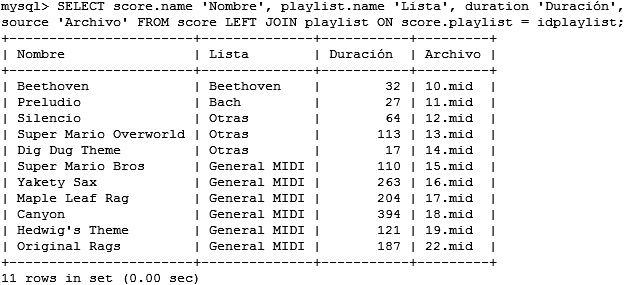
\includegraphics[width=\linewidth*3/4]{capitulo5/cap_sql}
		\par\end{centering}
	\smallskip
	\caption{\label{fig:cap_sql} Consulta de las piezas contenidas en la base de datos.}
\end{figure} 

\smallskip

\newpage

\section{Aplicaciones auxiliares}

He aquí la implementación de los programas diseñados para fines de verificación y soporte a módulos. Se trata en su mayoría de aplicaciones muy sencillas que cubrirán las funciones mínimas que no se han implantado en los subsistemas principales.

\subsection{Información de archivo MIDI}

Como se describió en la sección \ref{subsec:midinfo} de diseño, este programa tiene dos objetivos:

\begin{enumerate}
	\item Comprobar el funcionamiento del analizador \acrshort{MIDI}.
	\item Enviar la duración de una pieza a la interfaz \textit{web}.
\end{enumerate}

El programa recibe como argumento un \textbf{nombre de archivo}, que presuntamente corresponde a una partitura compatible, y utiliza la biblioteca implementada para analizar el archivo.

La naturaleza de la función en cuestión, \code{midi\_init()}, hace que el fichero sea analizado completamente, y recibamos una \textbf{estructura de datos} con toda la información extraída, a excepción de los mensajes exclusivos, no utilizados en este proyecto.

La aplicación devuelve al usuario una serie de datos tales como éstos:

\smallskip

\begin{figure}[H]
	\noindent \begin{centering}
		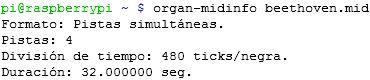
\includegraphics[width=\linewidth/2]{capitulo5/cap_midinfo}
		\par\end{centering}
	\smallskip
	\caption{\label{fig:cap_midinfo} Captura del visor de archivos MIDI.}
\end{figure} 

\smallskip

Existe una opción, \code{--duration}, que hace mostrar solamente la duración de la pieza, y la emite como un número \textbf{entero}, redondeando a la unidad. Ésta será la opción utilizada por la \textbf{interfaz \textit{web}} cuando insertemos un nuevo archivo.

En caso de \textbf{error de lectura}, se imprime un mensaje de error y se finaliza con ''\textbf{código 1}''. Esto además es útil al \textit{front-end} para garantizar que todo archivo subido corresponde efectivamente a una partitura \acrshort{MIDI}.

\subsection{Simulador de reproducción}
\label{subsec:simulador_reproduccion}

Este programa se diseñó para probar el planificador y la estructura de la salida, dos módulos que van de la mano y conforman el núcleo del demonio. En realidad es una \textbf{reimplementación} del prototipo del planificador que escribimos en Python, pero ahora trabaja con el planificador final.

La salida de datos, diseñada en la sección \ref{subsec:output} es una \textbf{interfaz} utilizada por el planificador, que evita la necesidad de modificarlo de manera alguna cuando nos movamos de un órgano a otro. Sus funciones públicas coinciden en su mayor parte con las instrucciones del \textbf{protocolo \acrshort{MIDI}}.

En este caso vamos a simular más exactamente el órgano de la Parroquia de la Encarnación de Santa Fe que el prototipo de la \acrshort{PCB}, en tanto que éste solo abordará 7 notas en cada canal. En resumen tendremos esta estructura:

\smallskip

\begin{center}
	\begin{tabular}{|l|l|l|l|}
		\hline \textbf{Pista} & \textbf{Extensión} & \textbf{Comienzo} & \textbf{Descripción} \\ 
		\hline 1 & 49 notas & 36 (\textit{Do-2}) & Teclado barroco \\
		\hline 2 & 49 notas & 36 (\textit{Do-2}) & Teclado romántico \\
		\hline 2 & 12 notas & 36 (\textit{Do-1}) & Pedalier \\
		\hline 2 & 49 notas & 36 (\textit{Do-4}) & Registros \\
		\hline 
	\end{tabular}
	\smallskip
	\captionof{table}{\label{tab:miditest_map} Asignación de notas en el simulador de reproducción.}
\end{center}

\smallskip

El simulador funcionará en consola, de forma que, en lugar de volcar la información en los puertos \acrshort{GPIO}, lo haremos hacia la \textbf{salida estándar}. A continuación mostramos una captura del programa:

\smallskip

\begin{figure}[H]
	\noindent \begin{centering}
		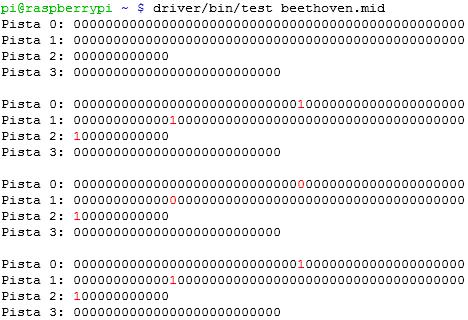
\includegraphics[width=\linewidth*3/4]{capitulo5/cap_miditest}
		\par\end{centering}
	\smallskip
	\caption{\label{fig:cap_miditest} Captura del visor de archivos MIDI.}
\end{figure} 

\smallskip

Como podemos comprobar, el planificador comienza realizando una función de limpieza (\textit{Panic}), escribiendo ceros en todas las notas. A continuación, de acuerdo a la partitura, se activan \textit{Mi-4} en la pista 0, \textit{Do-3} en la pista 1 y \textit{Do-1} en la pista 2 (pedal).

Después del tiempo correspondiente a una \textbf{negra}, se apagan las notas de las pistas 0 y 1 (teclados), manteniéndose la del pedal, para repetirse un instante después. En efecto, las dos primeras notas de la \textit{Oda a la Alegría} de Beethoven son \textbf{unísonas}.

Este es el único de los programas escritos en C que, por su naturaleza, \textbf{no se instalará} en el sistema de archivos, ya que no tiene más finalidad que depurar el sistema.

\subsection{Terminal del reproductor}.

De acuerdo a la sección \ref{subsec:terminal}, se implementaría un programa que nos permita comunicarnos con el demonio a través de la \textbf{consola}.

Esta aplicación abre un \textit{socket} cliente para comunicarse con el demonio, al que transmite las órdenes recibidas desde la consola, utilizando las mismas órdenes que especificamos en el protocolo.

\smallskip

\begin{figure}[H]
	\noindent \begin{centering}
		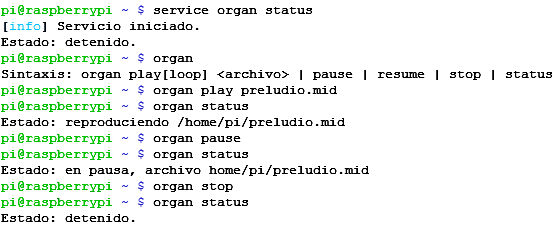
\includegraphics[width=\linewidth*3/4]{capitulo5/cap_terminal}
		\par\end{centering}
	\smallskip
	\caption{\label{fig:cap_terminal} Captura del controlador por terminal.}
\end{figure} 

\smallskip

\subsection{Comprobación de contraseña}
\label{subsec:aux_login}

Para autorizar la entrada a la interfaz gráfica, se ha decidido utilizar la seguridad de Linux, ya que utiliza la función de resumen (\textit{hash}) junto a una serie de \textit{bits} aleatorios (\textit{salt}) para almacenarla.

Nuestro programa utilizará la \textbf{\acrshort{API} de criptografía} de Linux para comprobar si una contraseña es válida. Ya que la clave no está almacenada como tal, sino solo un \textit{hash}, procederemos de la forma que sigue:

\begin{enumerate}
	\item La aplicación recibe un nombre de usuario y una contraseña.
	\item Buscamos en el sistema el usuario indicado, y obtenemos el \textit{hash} de su clave.
	\item Encriptamos la contraseña recibida con el mismo algoritmo y la misma sal.
	\item Comparamos ambos resúmenes: si coinciden, autentificamos al usuario.
\end{enumerate}

El programa devuelve un \textbf{código de error} si el usuario no existe o la clave no es válida. En este último caso, retrasa la ejecución 2 segundos, para dificultar un \textbf{ataque por fuerza bruta}.

El acceso al fichero de usuarios (\code{/etc/shadow}), utilizado por la utilidad de \textbf{autentificación}, requiere permisos de administrador. Aún así, tenemos la seguridad de que este programa no hará cambios en el sistema, y produce un \textbf{retraso} si recibe una contraseña que no coincide con el usuario. Con estas premisas instalamos la aplicación con la característica \textbf{\textit{setuid}}, que hace que se ejecute siempre con permisos de \textit{root}.

\subsection{Instalador del servidor}

El demonio incluye un \textit{Makefile} y un \textit{script} de preinstalación para ser compilado e instalado sin dificultad. La puesta en marcha de la interfaz y la base de datos requiere de una serie de pasos que, por simplicidad, reuniremos en un \textit{script} que lo haga automáticamente.

Las acciones que realiza son las siguientes:

\begin{enumerate}
	\item Instala el sistema MySQL, el servidor Apache y el lenguaje \acrshort{PHP}.
	\item Añade el usuario de Apache, \code{www-data}, al grupo \code{organ}.
	\item Genera el archivo de configuración del sitio \textit{web} desde una plantilla:
	
	\begin{enumerate}
		\item Establece un nombre del sitio ---que puede ser \textit{localhost}---.
		\item Selecciona el directorio raíz del sitio, y sus permisos.
		\item Crea un vínculo para la carpeta contenedora de archivos \acrshort{MIDI}.
	\end{enumerate}
	
	\item Ejecuta el archivo \acrshort{SQL} para crear la base de datos.
	\item Crea la carpeta raíz de la interfaz y el directorio de ficheros \acrshort{MIDI}.
\end{enumerate}

\newpage

\section{Resultado de la implementación}

Al término de la fase de implementación hemos obtenido todo el sistema \textit{software} en distintos módulos y aplicaciones, que darán a la \acrshort{PCB} todo el soporte especificado en los requisitos.

\subsection{Módulos}

Si bien el diseño del sistema ha distinguido entre \textit{front-end}, \textit{back-end} y base de datos, a la hora de implementarlo hemos separado el código en tres bloques:

\begin{description}
	\item[Controlador] Incluye el demonio y las aplicaciones auxiliares. En definitiva, todo aquello implementado en código para compilar.
	\item[Administrador] Comprende la interfaz \textit{web} y la base de datos.
	\item[Prototipos] Programas escritos para realizar pruebas sobre los módulos anteriores.
\end{description}

\subsubsection{Controlador}

Este bloque, que se encuentra en la rama \textbf{\textit{driver}} del desarrollo, contiene todo el código a compilar del demonio y los programas auxiliares. Se clasifican de la siguiente manera:

\smallskip

\begin{center}
	\begin{tabular}{|l|l|l|l|}
		\hline \multicolumn{1}{|c|}{\textbf{Aplicación}} & \multicolumn{1}{c|}{\textbf{Módulo}} & \multicolumn{1}{c|}{\textbf{Declaración}} & \multicolumn{1}{c|}{\textbf{Definición}} \\ 
		\hline \multirow{9}{*}{\textbf{Demonio}} & Base de datos & database.h & database.c \\
		\cline{2-4} & Salida & output.h & gpio.c \\
		\cline{2-4} & MIDI & midi.h & midi.c \\
		\cline{2-4} & Principal & & organd.c \\
		\cline{2-4} & Ingeniería & peripherals.h & peripherals.c \\
		\cline{2-4} & Planificador & player.h & player.c \\
		\cline{2-4} & Socket & socket.h & socket.c \\
		\cline{2-4} & UART & uart.h & uart.c \\
		\cline{2-4} & Constantes & values.h & \\
		\hline \textbf{Autentificación} & Principal & & login.c \\
		\hline \textbf{Información MIDI} & Principal & & midinfo.c \\
		\hline \multirow{2}{*}{\textbf{Simulador}} & Salida & (output.h) & monitor.c \\
		\cline{2-4} & Principal & & test.c \\
		\hline \textbf{Terminal} & Principal & & organ.c \\
		\hline 
	\end{tabular}
	\smallskip
	\captionof{table}{\label{tab:archivos_driver} Relación de módulos en el controlador.}
\end{center}

\smallskip

\subsubsection{Administrador}

El administrador incluye esencialmente todos los módulos relacionados con la programación \textit{web}, además de la base de datos. Los bloques de programación son los siguientes:

\smallskip

\begin{center}
	\begin{tabular}{|l|l|l|l|}
		\hline \multicolumn{1}{|c|}{\textbf{Módulo}} & \multicolumn{1}{c|}{\textbf{Vista}} & \multicolumn{1}{c|}{\textbf{Controlador}} & \multicolumn{1}{c|}{\textbf{Modelo}} \\ 
		\hline \multirow{2}{*}{\textbf{Portada}} & index.php & control.php & \\
		& index.js & & \\
		\hline \multirow{4}{*}{\textbf{Reproductor}} & player.php & control.php & \\
		& player.js & pause.php & \\
		& & resume.php & \\
		& & stop.php & \\
		\hline \multirow{2}{*}{\textbf{Listas}} & playlists.php & control.php & \\
		& playlists.js & & \\
		\hline \multirow{2}{*}{\textbf{Piezas}} & playlist.php & control.php & \\
		& playlist.js & & \\
		\hline \multirow{2}{*}{\textbf{Mando}} & remote.php & control.php & \\
		& remote.js & & \\
		\hline \textbf{Energía} & & control.php & \\
		\hline \textbf{Base de datos} & & & database.php \\
		\hline \textbf{Demonio} & & & driver.php \\
		\hline \textbf{Sesión} & & & session.php \\
		\hline \textbf{Traducción} & & & translator.php \\
		\hline 
	\end{tabular}
	\smallskip
	\captionof{table}{\label{tab:archivos_manager} Relación de módulos en el administrador.}
\end{center}

\smallskip

Además hemos añadido los siguientes archivos de soporte:

\smallskip

\begin{center}
	\begin{tabular}{|l|l|}
		\hline \multicolumn{1}{|c|}{\textbf{Recurso}} & \multicolumn{1}{c|}{\textbf{Archivos}}  \\ 
		\hline Plantillas HTML & templates.php \\
		\hline Constantes & values.php \\
		\hline Hoja de estilos & styles.css \\
		\hline \multirow{3}{*}{Traducciones} & english.xml \\
		& italian.xml \\
		& spanish.xml \\
		\hline Base de datos & organo.sql \\
		\hline 
	\end{tabular}
	\smallskip
	\captionof{table}{\label{tab:archivos_manager} Archivos de soporte al administrador.}
\end{center}

\smallskip

\subsection{Líneas de código}

Agrupamos todos los módulos y contamos las líneas de código para conocer la relación entre los 10 lenguajes utilizados y el grosor de cada uno de los tres bloques principales. Del código fuente no hemos tenido en cuenta las líneas vacías:

\smallskip

\begin{center}
	\begin{tabular}{|l|r|r|r|r|}
		\hline & \textbf{Controlador} & \textbf{Administrador} & \textbf{Prototipos} & \textbf{Total} \\ 
		\hline \textbf{C} & 2062 & & 498 & 2560 \\
		\hline \textbf{\acrshort{PHP}} & & 1051 & & 1051 \\
		\hline \textbf{Python} &  &  & 541 & 541 \\
		\hline \textbf{CSS} & & 460 & & 460 \\
		\hline \textbf{JavaScript} & & 263 & & 263 \\
		\hline \textbf{XML} & & 180 & & 180 \\
		\hline \textbf{Shell} & 122 & 36 & & 158 \\
		\hline \textbf{Makefile} & 86 &  & 10 & 96 \\
		\hline \textbf{SQL} & & 68 & & 68 \\
		\hline \textbf{Processing} & & & 25 & 25 \\
		\hline \textbf{Total} & 2270 & 2058 & 1074 & \textbf{5402} \\
		\hline 
	\end{tabular}
	\smallskip
	\captionof{table}{\label{tab:lineas} Recuento de líneas de código.}
\end{center}

\smallskip

Esta información se representa gráficamente de la siguiente manera:

\smallskip

\begin{figure}[H]
	\noindent \begin{centering}
		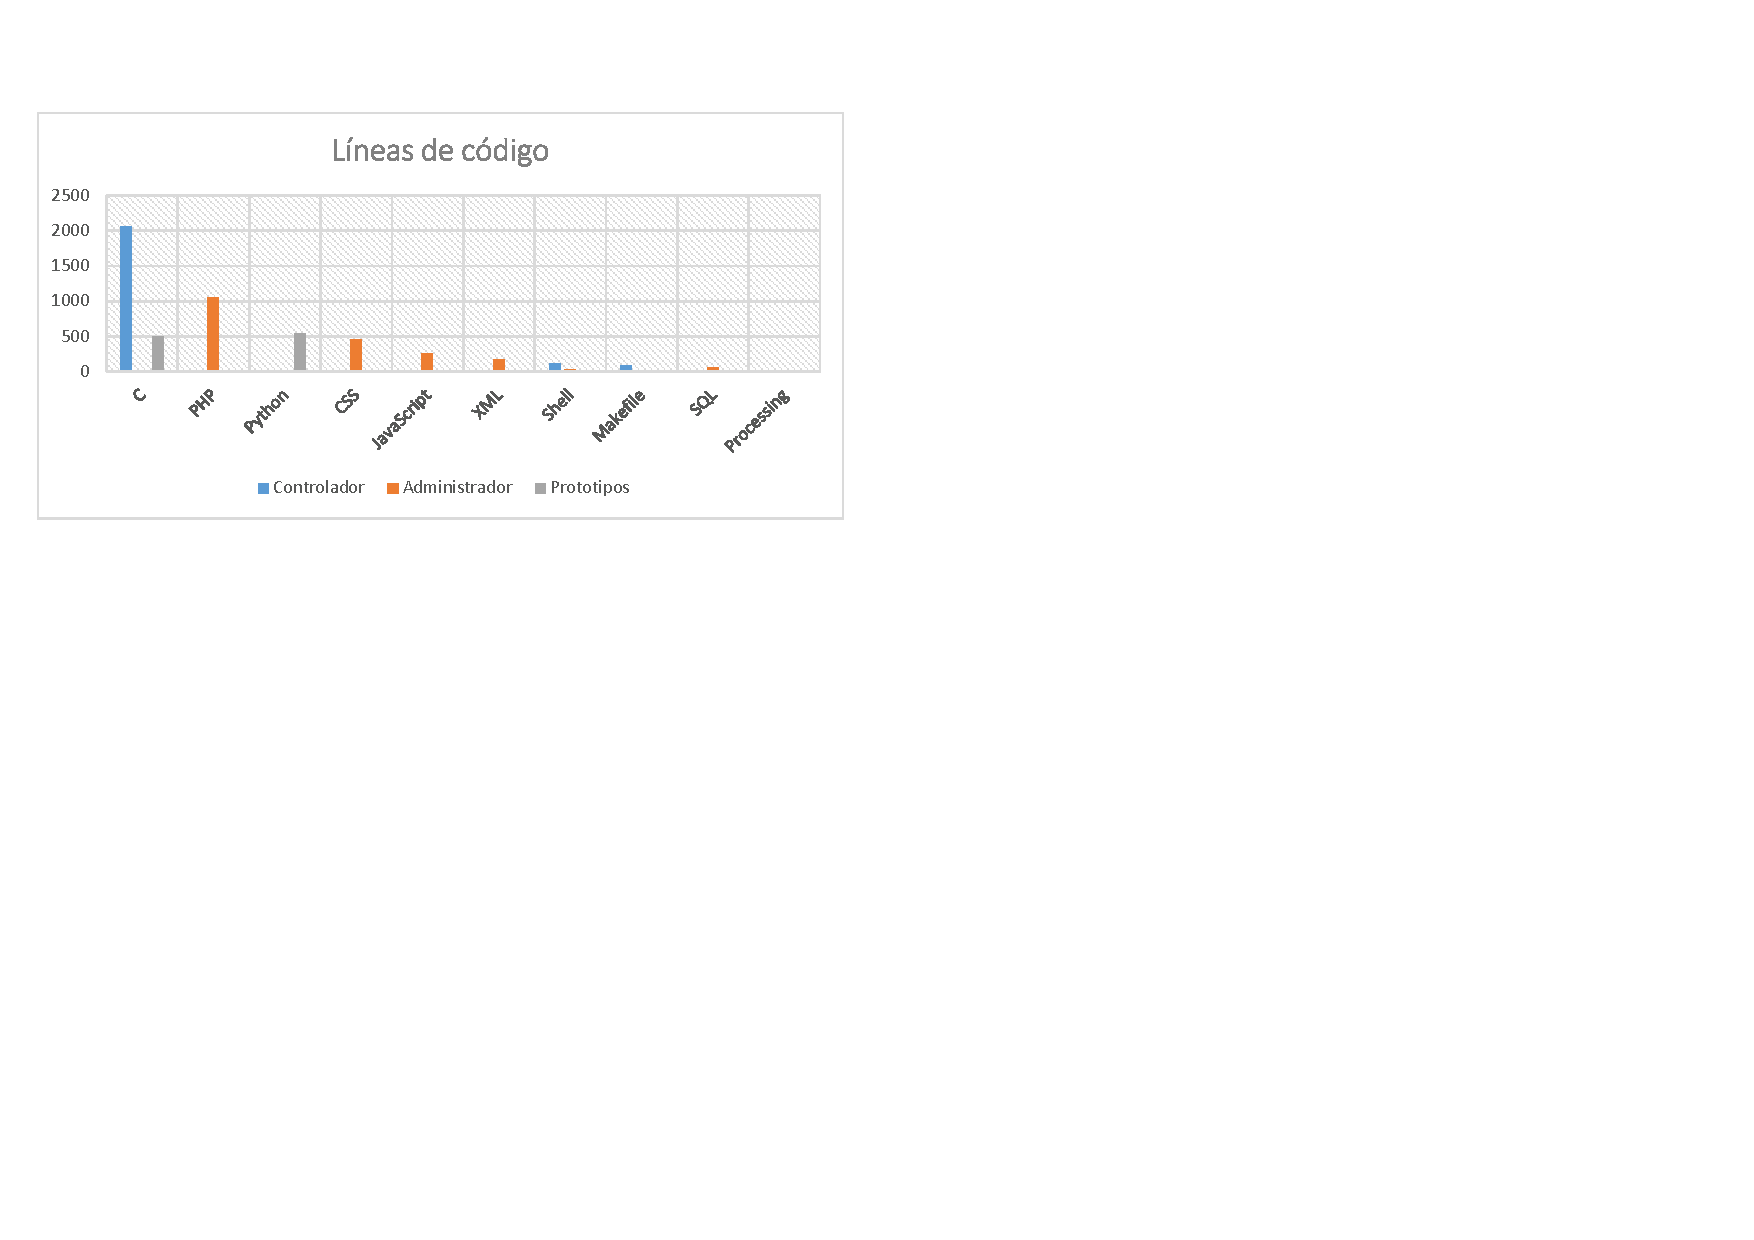
\includegraphics[clip=true,trim=10 340 410 50,width=\linewidth*3/4]{capitulo5/lineas}
		\par\end{centering}
	\smallskip
	\caption{\label{fig:lineas} Distribución del código fuente.}
\end{figure} 

\smallskip

Podemos ver que la mayor parte del código está en \textbf{lenguaje C} y pertenece al \textbf{controlador}, existiendo una cantidad menor de código para los prototipos. Le sigue \acrshort{PHP} en el administrador, mientras que Python ha sido el lenguaje más utilizado para prototipos.

Si agrupamos los datos en función de los bloques, obtenemos la siguiente gráfica:

\smallskip

\begin{figure}[H]
	\noindent \begin{centering}
		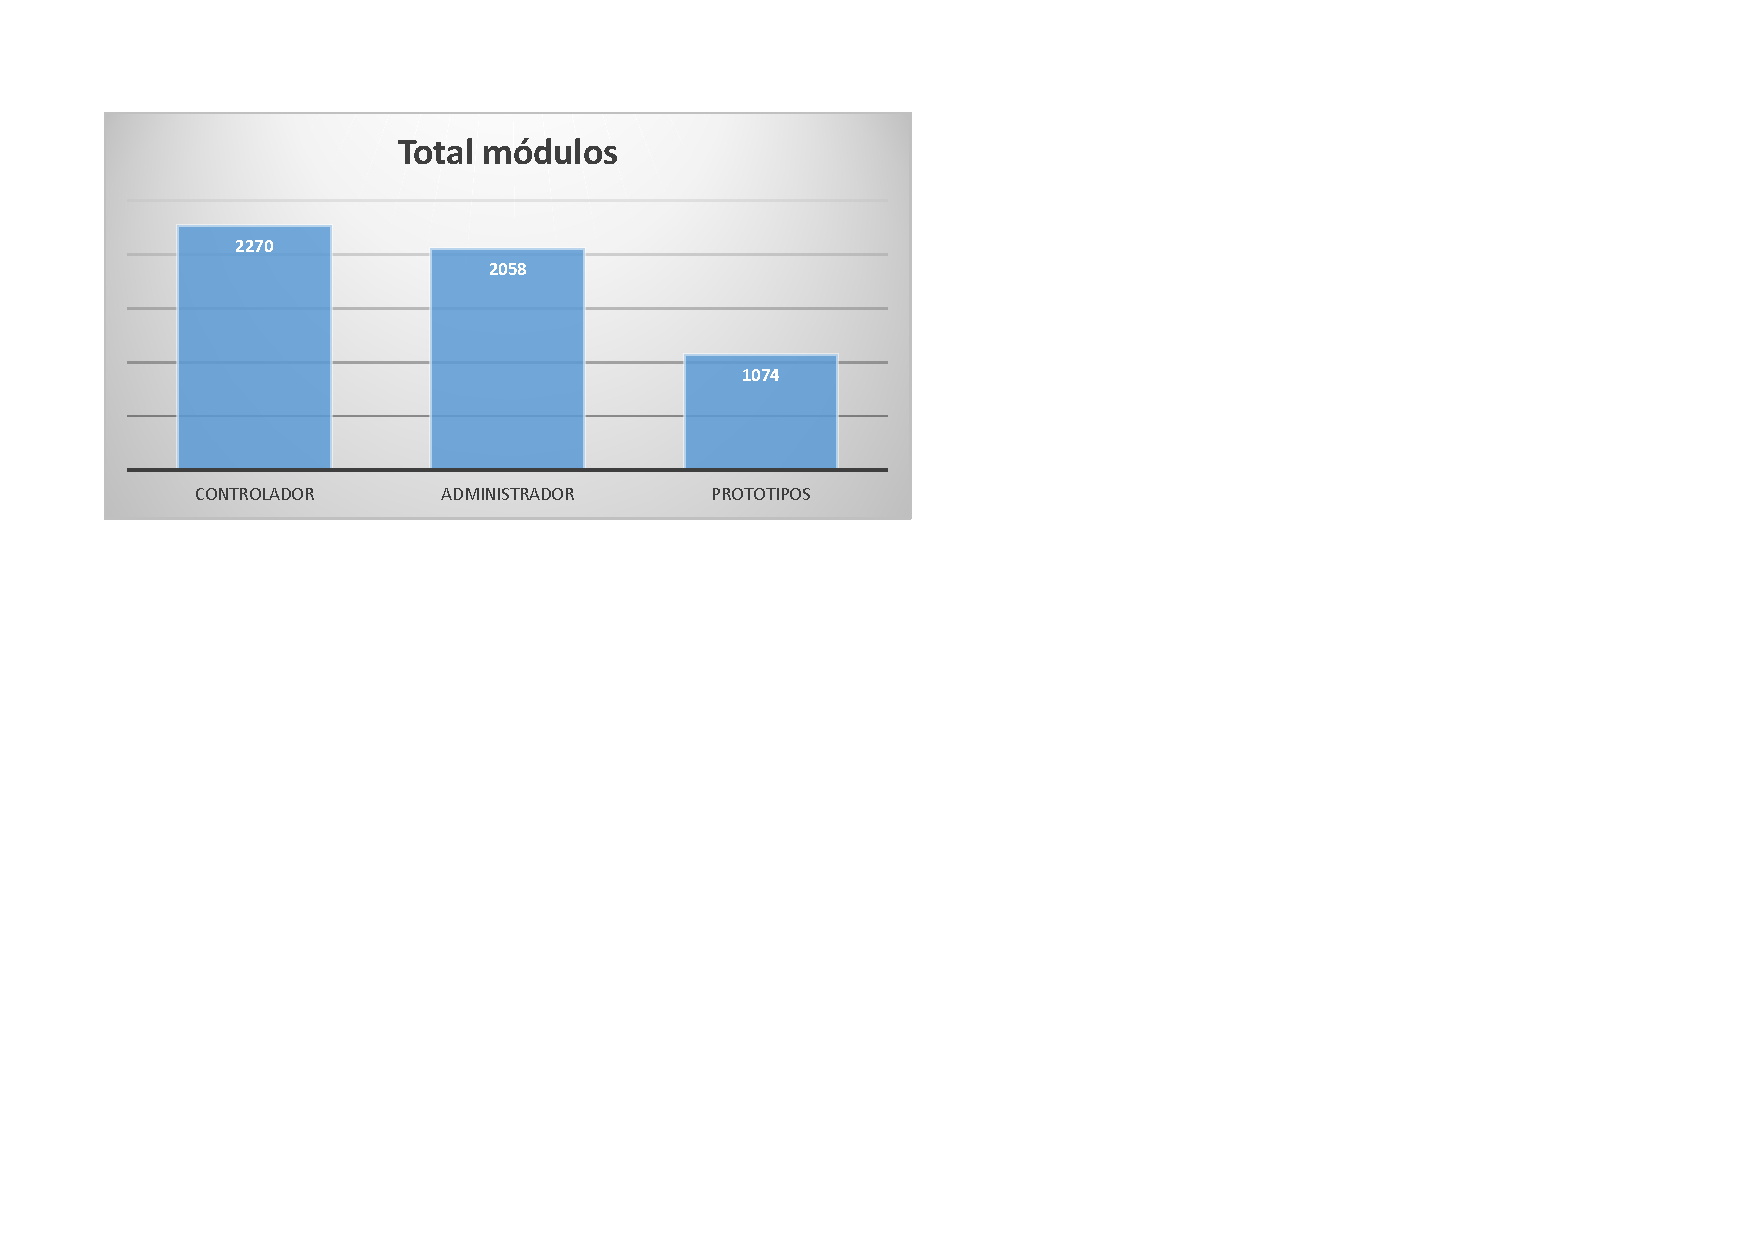
\includegraphics[clip=true,trim=10 340 410 50,width=\linewidth*3/4]{capitulo5/lineas_modulos}
		\par\end{centering}
	\smallskip
	\caption{\label{fig:lineas_modulos} Distribución del código fuente por módulos.}
\end{figure} 

\smallskip

El mayor coste en lo que a código se refiere ha sido el \textbf{controlador}, al que sigue de cerca el administrador.

Por último, mostramos la gráfica que agrupa las líneas de código en función del lenguaje:

\smallskip

\begin{figure}[H]
	\noindent \begin{centering}
		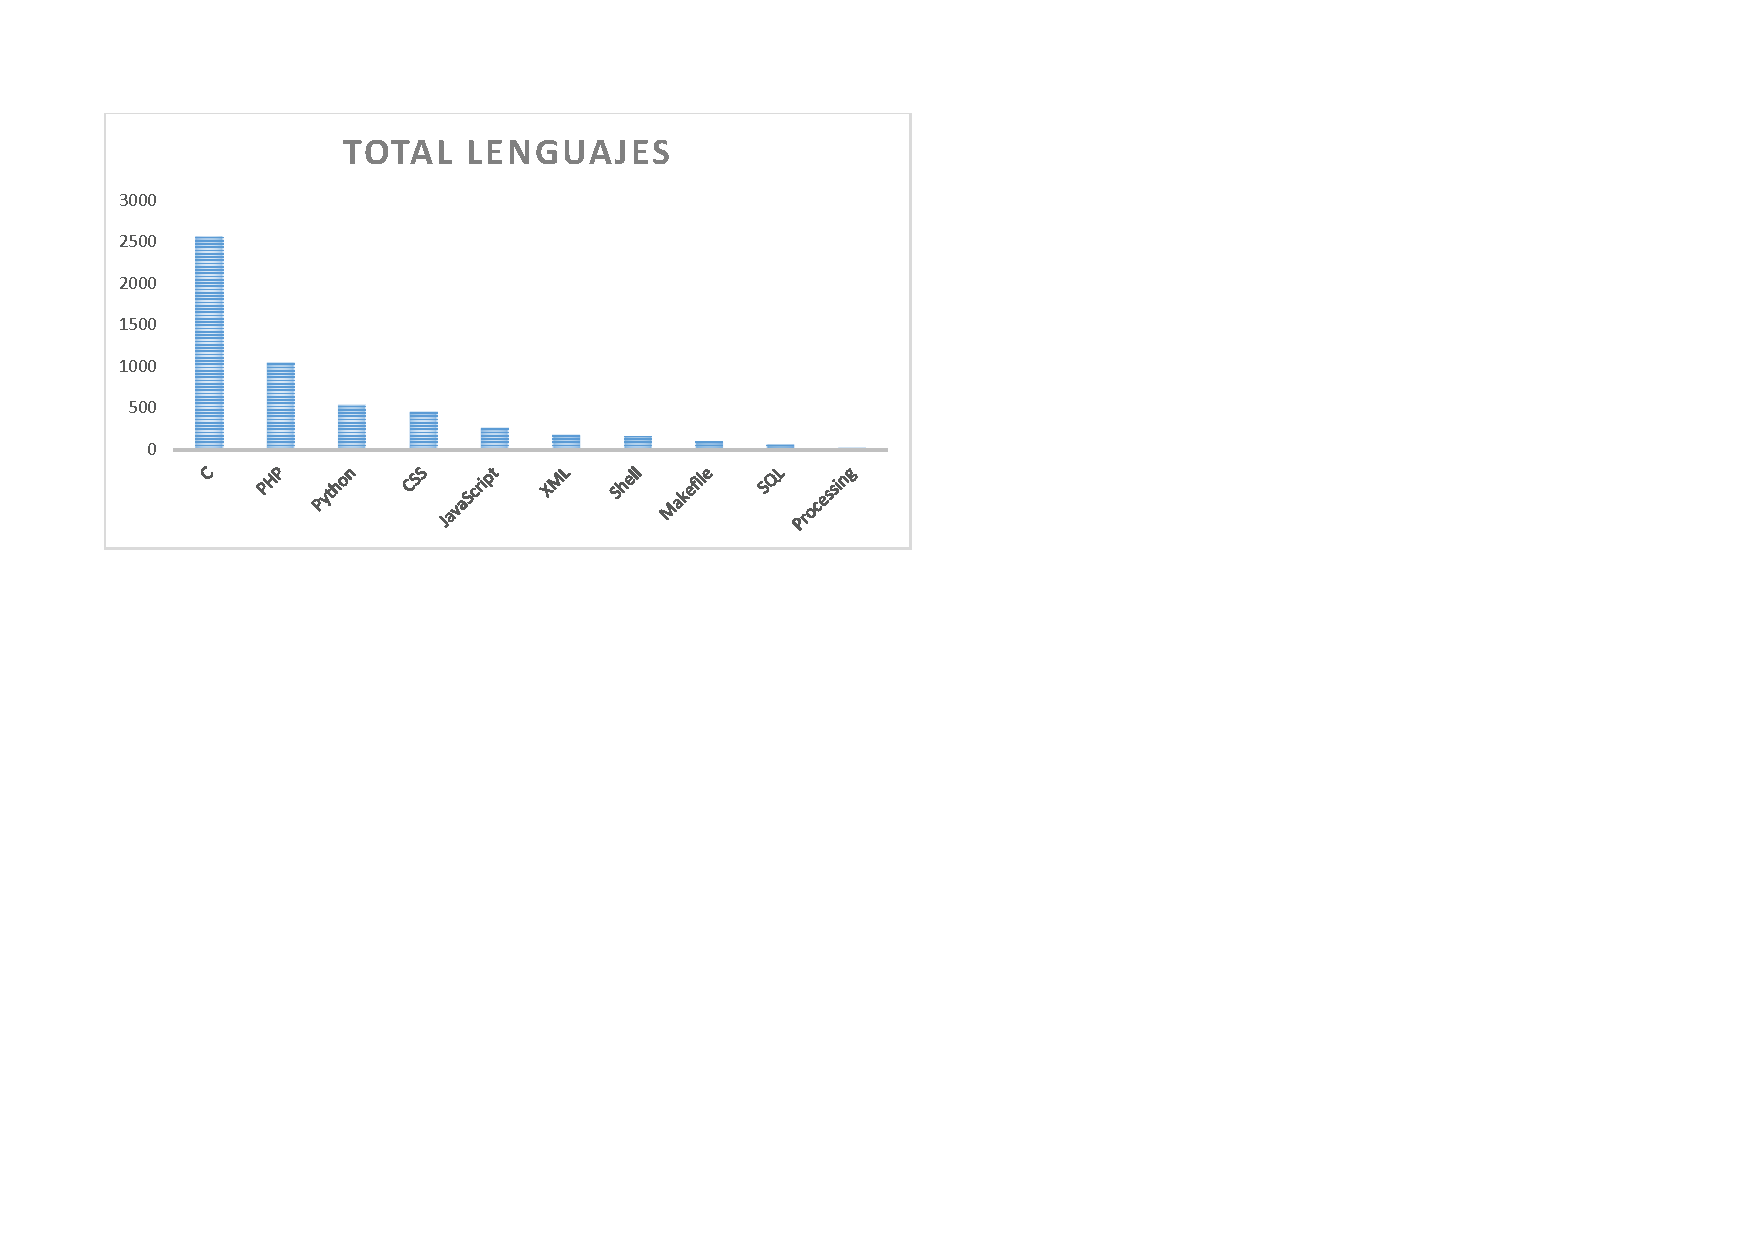
\includegraphics[clip=true,trim=10 330 400 50,width=\linewidth*3/4]{capitulo5/lineas_lenguajes}
		\par\end{centering}
	\smallskip
	\caption{\label{fig:lineas_lenguajes} Distribución del código fuente por lenguaje.}
\end{figure} 

\smallskip

El \textbf{lenguaje más utilizado} en este proyecto ha sido C con amplia diferencia. A pesar de que es un lenguaje de bajo nivel, con mayor coste de implementación y es fácil cometer errores con él, sobre todo utilizando aritmética de punteros, podremos ver en el capítulo que sigue que ha merecido la pena, tanto por su \textbf{eficiencia} como su capacidad de \textbf{modularización}.

\newpage
\clearpage{\pagestyle{empty}\cleardoublepage}